\documentclass[DynamicalBook]{subfiles}
\begin{document}
%


\setcounter{chapter}{5}%Just finished 5.

\chapter{Paradigms of Composition}\label{chapter.6} 

\section{Introduction}


Throughout this book so far, we seen dynamical systems modeled by state spaces exposing
variables and updating according to external parameters. This sort of dynamical
system is \emph{lens-based} --- systems are themselves lenses, and they compose by
lens composition. We might describe them as \emph{parameter-setting systems},
since we compose these systems by setting the parameters of some according to
the exposed state variables of others.

There are many parameter-setting doctrines: deterministic (distrete, continuous, measurable), differential (Euclidean, general), non-deterministic (possibilistic, probabilistic, cost-aware, etc.). From each doctrine $\dd$, we constructed a doubly indexed category $\Cat{Sys}_{\dd} : \Cat{Arena}_{\dd} \to \Cat{Cat}$, indexed by the double category of arenas in the doctrine $\dd$. This doubly indexed category organized the behaviors of the systems in doctrine $\dd$ (through the charts) and the ways that systems can be composed (through the lenses).

But composing systems through lenses is not the only way to model systems. In this section we will see two more ways of understanding what it means to be a system: the \emph{behavioral approach} to systems theory, which composes systems by sharing their exposed variables, and the \emph{diagrammatic approach} to systems theory, which composes diagrams describing systems by gluing together their exposed parts. In the behavioral approach (see \cite{sec:behavioral.approach}), systems are understood as (variable) sets of behaviors, some of which are exposed to their environment. These systems are composed by \emph{sharing} these exposed behaviors --- that is, by declaring the behaviors exposed by some systems to be the same. In the diagrammatic approach (see \cite{sec:diagram.approach}), systems are presented by diagrams formed by basic constituent parts, some of which are exposed to their environment. These systems are composed by gluing together their exposed parts.

In total, we will have three \emph{paradigms of composition} --- ways of thinking about what a \emph{theory of systems} could be, including how they are to be composed.

\begin{informal}\label{informal:paradigm}
 A \emph{paradigm of composition} is a particular way to answer the following questions about it means to be a \emph{systems theory}:
 \begin{itemize}
   \item What does it mean to be a system? Does it have a notion of states, or of behaviors? Or is it a diagram describing the way some primitive parts are organized?
   \item What should the interface of a system be?
   \item How can interfaces be connected in composition patterns?
  \item How are systems composed through composition patterns between their interfaces.
  \item What is a map between systems, and how does it affect their interfaces?
  \item When can maps between systems be composed along the same composition patterns as the systems.
  \end{itemize}
  \end{informal}

The \emph{parameter-setting paradigm} which has been the focus of the book so far answers these questions in the following way:
\begin{itemize}
  \item A system consists of a notion of how things can be, called the \emph{states}, and a notion of how things will change given how they are, called the \emph{dynamics}. In total, a system is a lens of the form $\lens{\update{S}}{\expose{S}} : \lens{T\State{S}}{\State{S}} \fromto \lens{\In{S}}{\Out{S}}$.
  \item The dynamics of a system can invovle certain \emph{parameters}, and \emph{expose} some variables of its state. The admissible parameters can depend on the variables being exposed. In total, an interface for a system is an arena $\lens{\In{S}}{\Out{S}}$.
  \item A composition pattern between interfaces says which exposed variables will be passed forward, and how the internal parameters should be set according to the external parameters and the exposed variables. That is, a composition pattern is a lens.
\item Systems are composed by setting the parameters of some according to the exposed variables of others. This is accomplished by lens composition.
  \item A map between systems is a function of state which respects observable behavior; it affects the interfaces as a chart.
  \item When we have a square in the double category of arenas between charts and lenses, we may compose maps of systems --- behaviors --- along the composition patterns represented by the lenses.
\end{itemize}

Formally, we have organized the answers to these questions in our definition of the doubly indexed category $\Cat{Sys}_{\dd} : \Cat{Arena}_{{\dd}} \to \Cat{Cat}$ in a given doctrine $\dd$. The doctrine further specifies these answers along the lines of \cref{informal.doctrine}. In general, there may be many doctrines in any paradigm of composition, further specifying what it really means to be a system within that systems theory. At the end of the day, however, we can expect to get a doubly indexed category, indexed by a double category of interfaces and sending each interface to the category of systems with that interface.

We will not give a fully formal definition of paradigm of composition in this book. Nevertheless, we can give a useful, semi-formal approximation: a paradigm of composition is any systematic way to product doubly indexed categories of systems.
\begin{semiformal}
  A \emph{paradigm of composition} is a systematic way to produce doubly indexed categories of systems. As a first pass, we might say a paradigm of composition $\paradigm{P}$ is a functor
  $$\Cat{Sys}^{\paradigm{P}} : \Cat{Doctrine}^{\paradigm{P}} \to \Cat{DblIx}$$
  from a category of $\paradigm{P}$-doctrines to the category of doubly indexed categories. To a $\paradigm{P}$-doctrine $\dd$, this associates a doubly indexed category
  $$\Cat{Sys}^{\paradigm{P}}_{{\dd}} : \Cat{Interface}^{{\paradigm{P}}}_{{\dd}} \to \Cat{Cat}$$
  indexed by a double category $\Cat{Interface}^{{\paradigm{P}}}_{{\dd}}$ of interfaces in the $\paradigm{P}$-doctrine $\dd$. This answers the questions of \cref{informal:paradigm} in the following ways:
  \begin{itemize}
          \item A system is an object of the category $\Cat{Sys}^{\paradigm{P}}_{\dd}(I)$.
          \item The interface of a system is an object of the double category $\Cat{Interface}^{{\paradigm{P}}}_{\dd}$.
          \item The composition patterns between interfaces are the vertical maps of $\Cat{Interface}^{{\paradigm{P}}}_{\dd}$.
          \item The systems are composed along a composition pattern $c : I_{1} \to I_{2}$ by the functor $\Cat{Sys}^{{\paradigm{P}}}_{\dd}(c) : \Cat{Sys}^{{\paradigm{P}}}_{\dd}(I_{1}) \to \Cat{Sys}^{{\paradigm{P}}}_{\dd}(I_{2})$.
          \item A map between systems $\sys{S}_{1} \in \Cat{Sys}^{{\paradigm{P}}}_{\dd}(I_{1})$ and $\sys{S}_{2} \in \Cat{Sys}^{{\paradigm{P}}}_{\dd}(I_{2})$ which acts as $f : I_{1} \to I_{2}$ (a horizontal map in $\Cat{Interface}^{{\paradigm{P}}}_{{\dd}}$) is an element of $\Cat{Sys}^{{\paradigm{P}}}_{\dd}(f)(\sys{S}_{1}, \sys{S}_{2})$.
          \item Maps can be composed along the same composition patterns as systems when there is a square  $\alpha$ of the appropriate signature in $\Cat{Interface}^{{\paradigm{P}}}_{\dd}$; the composite morphism is $\Cat{Sys}^{{\paradigm{P}}}_{\dd}(\alpha)(f)$.
  \end{itemize}
  \end{semiformal}

So far in this book, we have been working in the parameter-setting paradigm of composition given by lens composition.
\begin{definition}
The \emph{parameter-setting paradigm} $\paramsetting$ consists of the functor $\Cat{Sys}^{{\paramsetting}} : \Cat{Doctrine}^{\paramsetting} \to \Cat{DblIx}$ defined in \cref{thm.functoriality_system_construction}
  \end{definition}

  In this chapter, we will meet two other paradigms of composition: the \emph{behavioral approach} to systems theory which is characterized by span composition which we will call the \emph{variable sharing paradigm}, and the \emph{diagrammatic approach} to systems theory which is characterized by cospan composition which we will call the \emph{port-plugging paradigm}. These three paradigms --- parameter-setting, variable-sharing, and port-plugging --- capture a wide range of categorical systems theories in use. They are, however, by no means exhaustive.





\section{The Behavioral Approach to Systems Theory}\label{sec:behavioral.approach}

The parameter setting (lens-based) ways of thinking about systems are very useful for the \emph{design} of systems; we give
a minimal set of data ($\expose{}$ and $\update{}$) which in principle determines all behaviors, though it
might take some work to understand what behaviors are actually in the system
once we have set it up. But for the \emph{analysis} of dynamical systems, we
seek to prove properties about how systems behave. It helps if we
already know how a system behaves.

In the \emph{behavioral} approach to systems theory, pioneered by Jan Willems,
we take ``behavior'' as a primitive. In its most basic formulation, the behavioral
approach to systems theory considers a system $\Sys{S}$ to have a set
$\Set{B}(S)$ of state variables or ``behaviors''. The system also exposes some of these
state variables in a function $\expose{S} : \Set{B}_{\Sys{S}} \to \Set{V}_{\Sys{S}}$
to a set
$\Set{V}_{\Sys{S}}$ of possible values for these exposed variables.

In other words, we can see the behavioral approach to systems theory as taking
place in the doubly indexed category $\Cat{Vec} : \Cat{Matrix} \to \Cat{Cat}$
(or, as we'll see, some variants of it). An interface is a set $V$ of possible
values, and a system is a vector $B_v$ of sets varying over $v \in V$ --- the behaviors in
which the exposed variables take that given value. This might sound a bit
different from the idea of a function $\expose{S} : \Set{B}_{\Sys{S}} \to
\Set{V}_{\Sys{S}}$, but we can define the set $B_v$ to be $\expose{S}\inv(v)$,
and pass between these two notions. That is, we are making use of the
equivalence between the double categories of matrices and the double categories
of spans explored in \cref{sec.double_cat_of_matrices} to think of vectors of
sets of length $V$ as functions into $V$, and to think of matrices of sets as spans.

\begin{example}
Consider the Lotka-Volterra predator prey model $\Sys{LK}$ of
\cref{sec.differential_system} which is given by the following system of
differential equations:
\[
  \begin{cases}

\frac{dr}{dt} =  \const{b}_{\Sys{Rabbits}}
\cdot r - c_1 f r \\
\frac{df}{dt} = c_2 r f - \const{d}_{\Sys{Foxes}}
\cdot f
  \end{cases}
\]
Here, $r$ is the population of rabbits and $f$ is the population of foxes. In
\cref{ex:lotka.volterra.model}, we saw how to represent this as a differential
system $\lens{\rr^2}{\rr^2} \fromto \lens{\rr^2}{\ord{1}}$ with $\expose{LK} =
!$ the terminal map and
  \[
\update{\Sys{Rabbits}}( {r, (\const{b}_{\Sys{Rabbits}}, \const{d}_{\Sys{Rabbits}})} )
= \const{b}_{\Sys{Rabbits}} \cdot r - \const{d}_{\Sys{Rabbits}} \cdot r.
\]
For the behavioral approach, we would apply the doubly indexed functor
taking trajectories (from \cref{ex:trajectories.compositional.behavior}) to get
the behavioral point of view on the system $\Sys{LK}$:
\[
\Fun{Behave}_{\Sys{Time}}^{\littlelens{\rr^2}{\rr^2}}(\Sys{LK}) \in \Cat{Vec}\left(
  \Cat{Arena}_{\eucdiff}\left( \littlelens{\ord{1}}{\rr},\,
    \littlelens{\rr^2}{\rr^2} \right) \right).
\]
In other words, the set $\Set{B}_{\Sys{LK}}$ of behaviors is the set of trajectories together
with their charts in $\Sys{LK}$, and $\Set{V}_{\Sys{LK}}$ is the set of charts
for those trajectories --- that is, parameters varying in time. We can calculate
this from the definitions in \cref{thm.representable_discrete}:

\begin{align*}
  \Set{V}_{\Sys{LK}} &= \Cat{Arena}_{\eucdiff}\left( \littlelens{\ord{1}}{\rr},\,
                       \littlelens{\rr^2}{\ord{1}} \right)\\
                     &= \left\{
\lens{(\const{b}_{\Sys{Rabbits}}, \const{d}_{\Sys{Foxes}})}{!} : \lens{\ord{1}}{\rr} \rightrightarrows \lens{\rr^2}{\ord{1}}
                       \right\} \\
  &= \{((\const{b}_{\Sys{Rabbits}}, \const{d}_{\Sys{Foxes}})) : \rr \to \rr^4\}.\\
  \Set{B}_{\Sys{LK}} &= \left\{
    \begin{tikzcd}[ampersand replacement = \&, column sep = large]
      \lens{\rr}{\rr} \ar[r, shift left, dashed, "\lens{(\frac{dr}{dt}, \frac{df}{dt})}{(r, f)}"] \ar[r, dashed, shift right] \ar[d, shift right,
      "\lens{1}{\id}"'] \ar[d, shift left, leftarrow] \&
      \lens{\rr^2}{\rr^2} \ar[d, shift left, leftarrow,
      "\lens{\update{LK}}{\expose{LK}}"] \ar[d, shift right]\\
      \lens{\ord{1}}{\rr} \ar[r, dashed, shift right, "{\lens{(\const{b}_{\Sys{Rabbits}}, \const{d}_{\Sys{Foxes}})}{!}}"'] \ar[r, dashed,
      shift left] \& \lens{\rr^2}{\ord{1}}
    \end{tikzcd}
  \right\} \\
  &= \left\{((r, f),(\const{b}_{\Sys{Rabbits}}, \const{d}_{\Sys{Foxes}})) : \rr \to \rr^4 \middle| \begin{cases}
\frac{dr}{dt} =  \const{b}_{\Sys{Rabbits}}
\cdot r - c_1 f r \\
\frac{df}{dt} = c_2 r f - \const{d}_{\Sys{Foxes}}
\cdot f
  \end{cases}\right\}.\\
\end{align*}
and the map $\Set{B}_{\Sys{LK}} \to \Set{V}_{\Sys{LK}}$ is the projection
exposing the parameters:
\[
((r, f), (\const{b}_{\Sys{Rabbits}},
\const{d}_{\Sys{Foxees}})) \mapsto (\const{b}_{\Sys{Rabbits}},
\const{d}_{\Sys{Foxees}}).
\]
\end{example}
\begin{remark}
Note
that the parameters of the original differential system
$\Sys{LK}$ are considered as exposed variables of state in the behavioral
approach. This is because the behavioral approach composes systems by setting
exposed variables equal to eachother, so the parameters must be considered as
exposed variables so that they can be set equal to other variables.
\end{remark}

In this section, we'll a bit of how the behavioral approach to systems theory
works, and why we might want to do it. We'll begin with the main idea in
\cref{sec:behavioral.idea}. Then, in \cref{sec:behavioral.diagrams}, we'll see that in the behavioral
approach, there is a different sort of \emph{undirected} wiring diagram which
is used to compose systems
\[
\begin{tikzpicture}[unoriented WD, spacing=8pt, font=\tiny]
	\node[pack] (f1) {$\Sys{S}_1$};
	\node[pack, below right=1.7 and 1 of f1] (f3) {$\Sys{S}_2$};
	\node[pack, above right=1.7 and 1 of f3] (f2) {$\Sys{S}_3$};
	\node[pack, below right=1.7 and 1 of f2] (f4) {$\Sys{S}_4$};
	\node[outer pack, fit=(f1) (f4)] (outer) {};
	%
	\node[link] at ($(f1)!-.4!(outer)$) (t) {};
	\node[link] at ($(f1)!.5!(f3)$) (u) {};
	\node[link] at (f3 |-f1) (v){};
	\node[link] at ($(f3)!.5!(f2)$) (w) {};
	\node[link] at ($(w)!.3!(f4)$) (x) {};
	\node[link, below=.5 of f3] (y) {};
	\node[link] at ($(f4)!-.4!(outer)$) (z) {};
	%
	\draw (f1) -- (outer);
	\draw (v) -- (outer.north-|v);
	\draw (f4) -- (outer);
	\draw (f1) -- (v) -- (f2) -- (f3) -- (y);
	\draw (f1) -- (f3) to[bend right=10] (x);
	\draw (x) to [bend right=10] (f2);
	\draw (x) -- (f4);
\end{tikzpicture}
\]
The idea of these \emph{bubble diagrams} is that each wire carries an exposed variable of the
behaviors of each system. An connection between wires expresses an
equality of the variables carried on them. The wiring diagram as a whole shows
how the systems in it \emph{share} their variables. If lens-based systems are
all about setting parameters, the behavioral approach to systems theory using
spans is all about sharing variables.

Just as the wiring diagrams for lens based systems are the lenses in categories
of arities, the wiring diagrams for the span-based behavioral approach are spans
in the category of arities --- cospans of finite sets.

\subsection{The idea of the behavioral approach}\label{sec:behavioral.idea}

In the behavioral approach to systems theory, a system is a set (or variable
set, see \cref{sec:behavioral.types}) of \emph{behaviors} of the system. A
system exposes some variables of its behaviors. We can draw a behavioral system as a blob with wires dangling out of it which we
imagine are carrying the exposed variables. For example, the following system $\Sys{S}$
exposes three variables:
\[
\begin{tikzpicture}[unoriented WD, spacing=14pt]
	\node[pack] (f1) at (0, 0) {$\Sys{S}$};
	%
	\node at (1.5,0) (t1) {};
	\node at (-.75,1.3) (t2) {};
	\node at (-.75,-1.3) (t3) {};
	%
  \draw (f1) -- (t1);
  \draw (f1) -- (t2);
  \draw (f1) -- (t3);
\end{tikzpicture}
\]


As we have seen in
\cref{thm.representable_discrete}, we can get behavioral systems for any type of
behavior in any doctrine. One benefit of the behavioral approach is that all of
these different doctrines can be composed on the same footing: they're all just
behavioral systems.

Consider the following example borrowed from Willems'
\cite{Willems:Behavioral.Approach}. We consider a square bucket of water with
two pipes at the bottom through which the water can flow:
\[
  \Sys{Bucket}_1 =
  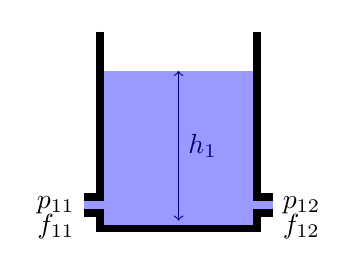
\begin{tikzpicture}[baseline=(center)]
    \fill[blue!40!white] (0, 0) rectangle (2,2);
    \fill[blue!40!white] (-.2, .2) rectangle (0.01,.4);
    \fill[blue!40!white] (2.2, .2) rectangle (1.99,.4);
    \draw[line width = .1cm] (0, 2.5) -- (0,.4) -- (-.2,.4);
    \draw[line width = .1cm] (-.2, .2) -- (0,.2) -- (0,0)
      -- (2,0) -- (2, .2) -- (2.2, .2);
    \draw[line width = .1cm] (2.2, .4) -- (2, .4) -- (2, 2.5);

    \draw[<->, blue!50!black] (1,.1cm) -- node[right] {$h_1$} (1, 2);
    \node[left] at (-.2, .3) {$p_{11}$};
    \node[below left] at (-.2, .3) {$f_{11}$};
    \node[right] at (2.2, .3) {$p_{12}$};
    \node[below right] at (2.2, .3) {$f_{12}$};

    \node (center) at (1, 1) {};
  \end{tikzpicture}
\]
The variable behaviors here are the pressures $p_{11}$ and $p_{12}$, the flows
$f_{11}$ and $f_{12}$, and the height of the water $h_1$. We suppose that these
quantities are related in the following ways:
\begin{align*}
  \frac{dh_1}{dt} &= F_1(h_1, p_{11}, p_{12}) \\
  f_{11} &= H_{11}(h_1, p_{11})\\
  f_{12} &= H_{12}(h_1, p_{12})
\end{align*}
for some functions $F_{1}$, $H_{11}$, and $H_{12}$. Therefore, the set of
behaviors is the set real valued functions of time which satisfy these laws:
\begin{equation}\label{eqn:bucket1.def}
\Set{B}_{\Sys{Bucket}_1} = \left\{ (h_1, f_{11}, f_{12}, p_{11}, p_{12}) : \rr
  \to \rr^5\, \middle|\,
\begin{aligned}
  \frac{dh_1}{dt} &= F_1(h_1, p_{11}, p_{12}) \\
  f_{11} &= H_{11}(h_1, p_{11})\\
  f_{12} &= H_{12}(h_1, p_{12})
\end{aligned}
\right\}
\end{equation}
We will suppose that we will only pump water to and from the bucket through the
pipes at the bottom. This means that we will only expose the variables
concerning those pipes.
\[
\Set{V}_{\Sys{Bucket}_1} = (\rr^4)^{\rr}
\]
and where
$$\expose{Bucket_1}(h_1, f_{11}, f_{12}, p_{11}, p_{12}) = (f_{11}, f_{12},
p_{11}, p_{12}).$$
We can bubble up the $\Sys{Bucket}_1$ system as the following bubble diagram:
\[
\begin{tikzpicture}[unoriented WD, spacing=14pt]
	\node[pack] (f1) at (0, 0) {$\mathsf{Bucket_1}$};
	%
	\node at (2,2) (t1) {};
	\node at (-2,2) (t2) {};
	\node at (-2,-2) (t3) {};
	\node at (2,-2) (t4) {};

  \node[above right] at (t1) {$p_{12}$};
  \node[above left] at (t2) {$p_{11}$};
  \node[below left] at (t3) {$f_{11}$};
  \node[below right] at (t4) {$f_{12}$};
	%
  \draw (f1) -- (t1);
  \draw (f1) -- (t2);
  \draw (f1) -- (t3);
  \draw (f1) -- (t4);
\end{tikzpicture}
\]
Each wire carries a variable element of $\rr \to \rr$, and the $\Sys{Bucket}_1$
system exposes four of such variables.

Now, suppose we had another bucket $\Sys{Bucket}_2$, governed by a similar set
of variables satisfying a similar set of laws, but with functions $F_{2}$,
$H_{21}$, and $H_{22}$ instead.
\[
  \Sys{Bucket}_2 =
  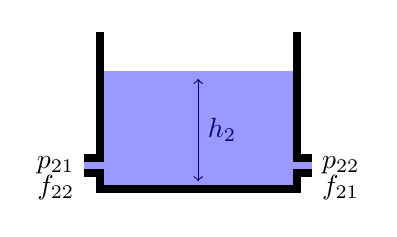
\begin{tikzpicture}[baseline=(center)]
    \fill[blue!40!white] (0, 0) rectangle (2.5,1.5);
    \fill[blue!40!white] (-.2, .2) rectangle (0.01,.4);
    \fill[blue!40!white] (2.7, .2) rectangle (2.49,.4);
    \draw[line width = .1cm] (0, 2) -- (0,.4) -- (-.2,.4);
    \draw[line width = .1cm] (-.2, .2) -- (0,.2) -- (0,0)
      -- (2.5,0) -- (2.5, .2) -- (2.7, .2);
    \draw[line width = .1cm] (2.7, .4) -- (2.5, .4) -- (2.5, 2);

    \draw[<->, blue!50!black] (1.25,.1cm) -- node[right] {$h_2$} (1.25, 1.4);
    \node[left] at (-.2, .3) {$p_{21}$};
    \node[below left] at (-.2, .3) {$f_{22}$};
    \node[right] at (2.7, .3) {$p_{22}$};
    \node[below right] at (2.7, .3) {$f_{21}$};

    \node (center) at (1.15, .75) {};
  \end{tikzpicture}
\quad = \quad
\begin{tikzpicture}[unoriented WD, spacing=14pt, baseline=(f1)]
	\node[pack] (f1) at (0, 0) {$\mathsf{Bucket_2}$};
	%
	\node at (2,2) (t1) {};
	\node at (-2,2) (t2) {};
	\node at (-2,-2) (t3) {};
	\node at (2,-2) (t4) {};

  \node[above right] at (t1) {$p_{21}$};
  \node[above left] at (t2) {$p_{22}$};
  \node[below left] at (t3) {$f_{21}$};
  \node[below right] at (t4) {$f_{22}$};
	%
  \draw (f1) -- (t1);
  \draw (f1) -- (t2);
  \draw (f1) -- (t3);
  \draw (f1) -- (t4);
\end{tikzpicture}
\]
Suppose we connect the two buckets up by the pipes at the bottom:
\[
  \Sys{Buckets} =
  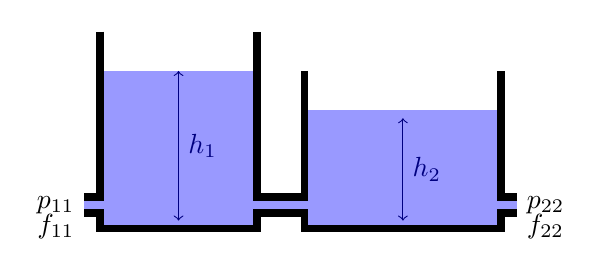
\begin{tikzpicture}[baseline=(center)]
    \fill[blue!40!white] (0, 0) rectangle (2,2);
    \fill[blue!40!white] (-.2, .2) rectangle (0.01,.4);
    \fill[blue!40!white] (2.4, .2) rectangle (1.99,.4);
    \draw[line width = .1cm] (0, 2.5) -- (0,.4) -- (-.2,.4);
    \draw[line width = .1cm] (-.2, .2) -- (0,.2) -- (0,0)
      -- (2,0) -- (2, .2) -- (2.4, .2);
    \draw[line width = .1cm] (2.4, .4) -- (2, .4) -- (2, 2.5);

    \draw[<->, blue!50!black] (1,.1cm) -- node[right] {$h_1$} (1, 2);
    \node[left] at (-.2, .3) {$p_{11}$};
    \node[below left] at (-.2, .3) {$f_{11}$};

    %%%%
    \node (center) at (0, 1) {};

    \fill[blue!40!white] (2.6, 0) rectangle (5.1,1.5);
    \fill[blue!40!white] (2.4, .2) rectangle (2.6,.4);
    \fill[blue!40!white] (5.3, .2) rectangle (5.09,.4);
    \draw[line width = .1cm] (2.6, 2) -- (2.6,.4) -- (2.4,.4);
    \draw[line width = .1cm] (2.4, .2) -- (2.6,.2) -- (2.6,0)
      -- (5.1,0) -- (5.1, .2) -- (5.3, .2);
    \draw[line width = .1cm] (5.3, .4) -- (5.1, .4) -- (5.1, 2);

    \draw[<->, blue!50!black] (3.85,.1cm) -- node[right] {$h_2$} (3.85, 1.4);
    \node[right] at (5.3, .3) {$p_{22}$};
    \node[below right] at (5.3, .3) {$f_{22}$};
  \end{tikzpicture}
\]
To express this combined system, we need that the pressures in the connected
pipes to be equal (since they are now one pipe), and we need the flows to be opposite (since any flow out of one
bucket goes into the other). That is, we need $p_{12} = p_{21}$ and $f_{12} +
f_{21} = 0$. All in all, the combined system has behaviors
\begin{equation}\label{eqn:combined.bucket.system}
  \Set{B}_{\Sys{Buckets}} = \left\{ \begin{aligned}
      (h_1, f_{11}, f_{12}, p_{11}, p_{12}) &: \rr \to \rr^5\\
      (h_2, f_{21}, f_{22}, p_{21}, p_{22}) &: \rr \to \rr^5\\
    \end{aligned}\,\middle|\,
\begin{aligned}
  \frac{dh_i}{dt} &= F_i(h_i, p_{i1}, p_{i2}) \\
  f_{i1} &= H_{i1}(h_i, p_{i1})\\
  f_{i2} &= H_{i2}(h_i, p_{i2})\\
  p_{12} &= p_{21} \\
  0 &= f_{12} + f_{21}
\end{aligned}
  \right\}
  \end{equation}
Meanwhile, the only variables which are exposed by $\Sys{Buckets}$ are the two
remaining open pipes, so
\begin{align*}
  \Set{V}_{\Sys{Buckets}} &= \rr \to \rr^4 \\
  \expose{Buckets}\left(\begin{aligned}
      (h_1, f_{11}, f_{12}, p_{11}, p_{12}) \\
      (h_2, f_{21}, f_{22}, p_{21}, p_{22})\\
    \end{aligned}  \right) &= (f_{11}, f_{22}, p_{11}, p_{22}).
\end{align*}

We can express the pattern of interconnection between $\Sys{Bucket}_1$ and
$\Sys{Bucket}_2$ as a bubble diagram to see precisely how $\Sys{Buckets}$ arises
as a composition of the two systems:
\begin{equation}\label{eqn:bucket.diagram}
\begin{tikzpicture}[unoriented WD, spacing=14pt, baseline=(f1)]
	\node[pack] (f1) at (0, 0) {$\mathsf{Buckets}$};
	%
	\node[] at (2,2) (t1) {};
	\node[] at (-2,2) (t2) {};
	\node[] at (-2,-2) (t3) {};
	\node[] at (2,-2) (t4) {};

  \node[above right] at (t1) {$p_{22}$};
  \node[above left] at (t2) {$p_{11}$};
  \node[below left] at (t3) {$f_{11}$};
  \node[below right] at (t4) {$f_{22}$};
	%
  \draw (f1) -- (t1);
  \draw (f1) -- (t2);
  \draw (f1) -- (t3);
  \draw (f1) -- (t4);
\end{tikzpicture}
\quad = \quad
\begin{tikzpicture}[unoriented WD, baseline = (plus)]
	\node[pack] (f1) {$\Sys{Bucket}_1$};
	\node[circle, draw, below right=1.7 and 1 of f1] (plus) {$+$};
	\node[pack, above right=1.7 and 1 of plus] (f2) {$\Sys{Bucket}_2$};
  \node[circle, draw, below = 1.7 of plus] (zero) {$0$};
	\node[outer pack, fit={ (f1) (plus) (f2) (zero) }] (outer) {};
	%
  \node[link, above = 6 of plus] (link) {};
 	%
  \draw (f1) to[out = 45, in = 180] (link);
  \draw (f2) to[out = 135, in = 0] (link);
  \draw (f1) to[out = 315, in=135] (plus);
  \draw (f2) to[out = 225, in=45] (plus);
  \draw (zero) -- (plus);
  \draw (f1) to[out=135, in=135] (outer);
  \draw (f1) to[out=225, in=225] (outer);
  \draw (f2) to[out=45, in=45] (outer);
  \draw (f2) to[out=315, in=315] (outer);
\end{tikzpicture}
\end{equation}

When the wires are connected in this diagram, they express an \emph{equality}
between their exposed variables. The top connection signifies that $p_{12} =
p_{21}$. The bubbled up $+$ signifies a relation (other than equality): it says
that the sum of the variables on the top two wires equals the third wire. We set
that third wire to be constant at $0$, so in total we get the relation that
$f_{12} + f_{21} = 0$.

We can analyze this composition of the systems $\Sys{Bucket}_1$ and
$\Sys{Bucket}_2$ in terms of the doubly indexed category
$\Cat{Vec} : \Cat{Matrix} \to \Cat{Cat}$, or rather the equivalent doubly
indexed category $\Cat{Set}/(-) : \Cat{Span}(\Cat{Set}) \to \Cat{Cat}$. To see how this works, let's remember how we compose
lens based systems in a given doctrine $\dd$.

Let's compose the $\Sys{Clock}$ and $\Sys{Meridian}$ systems into the
$\Sys{ClockWithDisplay}$ system from \cref{ex.ClockWithDisplay}.
\begin{equation}\label{eqn:example.diag.clockwithdispl}
\begin{tikzpicture}[oriented WD, every fit/.style={inner xsep=\bbx, inner ysep=\bby}, bbx = .3cm, bby =.3cm, bb min width=.5cm, bb port length=2pt, bb port sep=1, baseline=(Y.center)]
	\node[bb={1}{1}, fill=blue!10] (X1) {$\Sys{Meridian}$};
  	\node[bb={0}{1}, fill=blue!10, below=2 of X1] (X2) {$\Sys{Clock}$};
	\node[bb={0}{2}, fit={($(X1.north west)+(-2,1)$) ($(X1.north east)+(2,1)$) ($(X2.south)+(0,-3)$)}] (Y) {};
  \node[above=0pt of Y.south] (Label) {$\Sys{ClockWithDisplay}$};
	\draw (X1_out1) to (Y_out1);
  \draw let \p1=(X1.south west), \p2=(X2.north east), \n1=\bbportlen, \n2=\bby in
    (X2_out1) to[in=0] (\x2 + \n1, \y2 + \n2) -- (\x1 - \n1, \y2 + \n2) to[out=180] (X1_in1);
  \draw (X2_out1) to (Y_out2);
	\draw[label]
		node [right=2pt of Y_out1] {$\Set{a.m./p.m.}$}
		node [right=2pt of Y_out2] {$\Set{Hour}$}
		;
\end{tikzpicture}
\quad=\quad
\begin{tikzpicture}[oriented WD, every fit/.style={inner xsep=\bbx, inner ysep=\bby}, bbx = .3cm, bby =.3cm, bb min width=.5cm, bb port length=0, bb port sep=1, baseline=(Y.center)]
	\node[bb={1}{1}, fill=blue!10] (X1) {$\Sys{Meridian}$};
  	\node[bb={0}{1}, fill=blue!10, below=2 of X1] (X2) {$\Sys{Clock}$};

  \node[dashed, bb={1}{2}, fit={($(X1.north west)+(-2,1)$) ($(X1.north east)+(2,1)$) ($(X2.south)+(0,-3)$)}]  (Mid) {};
  \node[above=0pt of Mid.south] (Label) {$\Sys{Meridian} \otimes \Sys{Clock}$};

	\node[bb={0}{2}, fit={($(Mid.north west)+(-3,1)$) ($(Mid.north east)+(2,1)$) ($(Mid.south)+(0,-5)$)}] (Y) {};
  \node[above=0pt of Y.south] (Label) {$\lens{w^{\sharp}}{w}$};

	\draw (X1_out1) to (Mid_out1|-X1_out1);
  \draw (X2_out1) to (Mid_out2|-X2_out1) coordinate (Midout);
  \draw (Mid_in1|-X1_in1) coordinate (Midin) to (X1_in1);

  \draw (Mid_out1|-X1_out1) to (Y_out1|-X1_out1);
  \draw (Mid_out2|-X2_out1) to (Y_out1|-X2_out1);


  \draw let \p1=(Mid.south east), \p2=(Mid.south west), \n1=\bbportlen, \n2=\bby in
    (Midout) to[out=0, in=0] (\x1 + \n1, \y1-\n2) -- (\x2 - \n1, \y1 - \n2) to[out=180, in=180] (Midin);

	\draw[label]
		node [right=2pt of Y_out1|-X1_out1] {$\Set{a.m./p.m.}$}
		node [right=2pt of Y_out2|-X2_out1] {$\Set{Hour}$}
		;
\end{tikzpicture}
\end{equation}

We begin with
$\Sys{Clock}$, which is in the category
$\Cat{Sys}_{\determ}\lens{\ord{1}}{\Set{Hour}}$ of deterministic
systems with interface $\lens{\ord{1}}{\Set{Hour}}$, and $\Sys{Meridian}$, which
is in the category $\Cat{Sys}_{\determ}\lens{\Set{Hour}}{\Set{a.m./p.m.}}$ of
deterministic systems with interface $\lens{\Set{Hour}}{\Set{a.m./p.m.}}$. We
then form their parallel product $\Sys{Meridian} \otimes \Sys{Clock}$, which is
in $\Cat{Sys}_{\determ}\lens{\1\times\Set{Hour}}{\Set{a.m./p.m.} \times
  \Set{Hour}}$. The wiring diagram itself
\begin{equation}
\begin{tikzpicture}[oriented WD, every fit/.style={inner xsep=\bbx, inner ysep=\bby}, bbx = .3cm, bby =.3cm, bb min width=2cm, bb port length=0, bb port sep=2, baseline=(Y.center)]
  \node[bb={1}{2}, fill=blue!10]  (Mid) {};

	\node[bb={0}{2}, fit={($(Mid.north west)+(-3,1)$) ($(Mid.north east)+(2,1)$) ($(Mid.south)+(0,-5)$)}] (Y) {};
  \node[above=0pt of Y.south] (Label) {$\lens{w^{\sharp}}{w}$};


  \draw (Mid_out1) to (Y_out1|-Mid_out1);
  \draw (Mid_out2) to (Y_out1|-Mid_out2);


  \draw let \p1=(Mid.south east), \p2=(Mid.south west), \n1=\bbportlen, \n2=\bby in
    (Mid_out2) to[out=0, in=0] (\x1 + \n1, \y1-\n2) -- (\x2 - \n1, \y1 - \n2) to[out=180, in=180] (Mid_in1);

	\draw[label]
		node [right=2pt of Y_out1|-Mid_out1] {$\Set{a.m./p.m.}$}
		node [right=2pt of Y_out2|-Mid_out2] {$\Set{Hour}$}
		;
\end{tikzpicture}
\end{equation}
is a lens
$$\lens{w^{\sharp}}{w} : \lens{\1\times\Set{Hour}}{\Set{a.m./p.m.} \times \Set{Hour}} \leftrightarrows \lens{\ord{1}}{\Set{a.m./p.m.} \times \Set{Hour}}.$$
That is, it is a vertical arrow in the double category $\Cat{Arena}_{\determ}$
of arenas in the deterministic doctrine. The doubly indexed category $\Cat{Sys}_{\determ}
: \Cat{Arena}_{\determ} \to \Cat{Cat}$ furnishes us with a functor
$$\Cat{Sys}_{\determ}\littlelens{w^{\sharp}}{w} : \Cat{Sys}_{\determ}\lens{\1\times\Set{Hour}}{\Set{a.m./p.m.} \times
  \Set{Hour}} \to \Cat{Sys}_{\determ}\lens{\ord{1}}{\Set{a.m./p.m.} \times \Set{Hour}}$$
Despite its formidible name, this functor is just given by composing in
$\Cat{Arena}_{\determ}$ with the lens $\lens{w^{\sharp}}{w}$. We then apply this
functor to $\Sys{Meridian} \otimes \Sys{Hour}$ to get the composite system $\Sys{ClockWithDisplay}$:
$$\Sys{ClockWithDisplay} = \Cat{Sys}_{\determ}\littlelens{w^{\sharp}}{w}(\Sys{Meridian} \otimes \Sys{Hour}).$$

This story is mirrored in the behavioral approach to systems theory, except
instead of working with the doubly indexed category $\Cat{Sys}_{\dd} :
\Cat{Arena}_{\dd} \to \Cat{Cat}$, we work in the doubly indexed category
$\Cat{Vec} : \Cat{Matrix} \to \Cat{Cat}$ --- or, rather, the equivalent doubly
indexed category $\Cat{Set}/(-) : \Cat{Span}(\Cat{Set}) \to \Cat{Cat}$.

We begin with the systems $\Sys{Bucket}_1$ and $\Sys{Bucket}_2$, both in
$\Cat{Set}/(\rr^4)^{\rr}$; that is, $\Sys{Bucket}_1$ is identified with the map
$\expose{Bucket_1} : \Set{B}_{\Sys{Bucket_1}} \to (\rr^4)^{\rr}$, and the same
for $\Sys{Bucket_2}$. We then form the parallel product of these systems,
which in this case is given by their cartesian product
\[
\expose{\Sys{Bucket}_1} \times \expose{\Sys{Bucket}_2} :
\Set{B}_{\Sys{Bucket}_1} \times \Set{B}_{\Sys{Bucket}_2} \to (\rr^4)^{\rr}
\times (\rr^4)^{\rr}
\]
which is an object of $\Cat{Set}/((\rr^4)^{\rr} \times (\rr^4)^{\rr})$. Now, the
wiring diagram
\[
  W =
\begin{tikzpicture}[unoriented WD, baseline = (plus)]
	\node[pack] (f1) {$\phantom{\Sys{Bucket}_1}$};
	\node[circle, draw, below right=1.7 and 1 of f1] (plus) {$+$};
	\node[pack, above right=1.7 and 1 of plus] (f2) {$\phantom{\Sys{Bucket}_2}$};
  \node[circle, draw, below = 1.7 of plus] (zero) {$0$};
	\node[outer pack, fit={ (f1) (plus) (f2) (zero) }] (outer) {};
	%
  \node[link, above = 6 of plus] (link) {};
  \node[above = .1cm of link] {$a_1$};
 	%
  \draw (f1) to[out = 45, in = 180] (link);
  \draw (f2) to[out = 135, in = 0] (link);
  \draw (f1) to[out = 315, in=135] node[below left] {$a_2$} (plus);
  \draw (f2) to[out = 225, in=45] node[below right] {$a_3$} (plus);
  \draw (zero) -- node[left] {$a_4$}(plus);
  \draw (f1) to[out=135, in=135] node[below left] {$a_5$} (outer);
  \draw (outer) to[in=225, out=225] node[below left] {$a_6$}(f1);
  \draw (f2) to[out=45, in=45]node[left] {$a_7$} (outer);
  \draw (f2) to[out=315, in=315] node[right] {$a_8$}(outer);
\end{tikzpicture}
\]
may be described as a span of sets,
\[\begin{tikzcd}
	& W \\
	{(\rr^4)^{\rr} \times (\rr^4)^{\rr}} && {(\rr^4)^{\rr}}
	\arrow["{w_1}"', from=1-2, to=2-1]
	\arrow["{w_2}", from=1-2, to=2-3]
\end{tikzcd}\]
which is to say a vertical arrow in
$\Cat{Span}(\Cat{Set})$.
We'll explain how bubble diagrams correspond to spans in a more systematic way in
\cref{sec:behavioral.diagrams}, but for now we can define $W$ as follows:
  \begin{equation}\label{eqn:buckets.span.def}
    W = \left\{ (a_i)_{1 \leq i \leq 8} : \rr \to \rr^8 \,\middle|\, \begin{aligned}
        a_2 + a_3 &= a_4 \\
        a_4 &= 0
\end{aligned}\right\} \\
  \end{equation}
  \begin{align*}
    w_1((a_i)_{1 \leq i \leq 8}) &= ((a_6, a_2, a_5, a_1), (a_3, a_8, a_1, a_7))\\
    w_2((a_i)_{1 \leq i \leq 8}) &= (a_6, a_7, a_5, a_8)
                                   \end{align*}

We then compose $\Sys{Bucket}_1$ and $\Sys{Bucket}_2$ into the composite
$\Sys{Buckets}$ by applying $\Cat{Vec}(W)$ to $\Sys{Bucket_1} \times \Sys{Bucket_2}$:
\[
\Sys{Buckets} = \Cat{Vec}(W)(\Sys{Bucket_1} \times \Sys{Bucket_2}).
\]
This means composing with $W$ in the category of spans. Recall that we can see
the map $\expose{\Sys{Bucket}_1} \times \expose{\Sys{Bucket}_2} :
\Set{B}_{\Sys{Bucket}_1} \times \Set{B}_{\Sys{Bucket}_2} \to (\rr^4)^{\rr}
\times (\rr^4)^{\rr}$ as a span from $\ord{1}$ to $(\rr^4)^{\rr} \times
(\rr^4)^{\rr}$. Composing with $W$ therefore means we have the following
pullback diagram:
\begin{equation}\label{eqn:pullback.composition.of.systems}
\begin{tikzcd}
	& {\Set{B}_{\Sys{Buckets}}} \\
	{\Set{B}_{\Sys{Bucket}_1} \times \Set{B}_{\Sys{Bucket_2}}} && W \\
	& {(\rr^4)^{\rr} \times (\rr^4)^{\rr}} && {(\rr^4)^{\rr}}
	\arrow["{w_1}"', from=2-3, to=3-2]
	\arrow["{w_2}", from=2-3, to=3-4]
	\arrow["{\expose{Bucket_1} \,\times\, \expose{Bucket_2}}"', from=2-1, to=3-2]
	\arrow[dashed, from=1-2, to=2-1]
	\arrow[dashed, from=1-2, to=2-3]
	\arrow["\ulcorner"{anchor=center, pos=0.125, rotate=-45}, draw=none, from=1-2, to=3-2]
	\arrow["{\expose{Buckets}}", bend left = 30, from=1-2, to=3-4]
\end{tikzcd}
\end{equation}

Quite explicitly, this defines $\Set{B}_{\Sys{Buckets}}$ to be the set
\begin{equation} \label{eqn:combined.bucket.system.2}
\Set{B}_{\Sys{Buckets}} = \left\{ \begin{aligned} (h_1, f_{11}, f_{12}, p_{11}, p_{12}) &: \rr \to \rr^5\\
      (h_2, f_{21}, f_{22}, p_{21}, p_{22}) &: \rr \to \rr^5\\ (a_i)_{1 \leq i
        \leq 8} &: \rr \to \rr^8 \end{aligned} \,
  \middle|\, \begin{aligned}\frac{dh_i}{dt} &= F_i(h_i, p_{i1}, p_{i2}) \\
  f_{i1} &= H_{i1}(h_i, p_{i1})\\
  f_{i2} &= H_{i2}(h_i, p_{i2})\\
        a_2 + a_3 &= a_4 &
        a_4 &= 0\\
        p_{11} &= a_5  &
        f_{11} &= a_6 \\
        p_{12} &= a_1  &
        f_{12} &= a_2 \\
        p_{21} &= a_1  &
        f_{21} &= a_3 \\
        p_{22} &= a_7  &
        f_{22} &= a_8
\end{aligned} \right\}
\end{equation}
At first glance, this is quite a bit larger than the definition of
$\Set{B}_{\Sys{Buckets}}$ we gave in \cref{eqn:combined.bucket.system}. But most
of the equations here are setting the $f$s and $p$s from each $\Sys{Bucket}_i$
to be equal to the $a$s coming form the wiring diagram $W$. When the dust has
settled, the two definitions are equivalent --- which is to say more precisely
that they are isomorphic in the category $\Cat{Vec}((\rr^4)^{\rr})$.

\begin{exercise}
  Describe explicitly the isomorphism between the definitions of
  $\Set{B}_{\Sys{Bucket}}$ in \cref{eqn:combined.bucket.system} and
  \cref{eqn:combined.bucket.system.2}. Check that this isomorphism commutes with
  the two definitions of $\expose{Buckets}$ as well.
\end{exercise}

A crucial feature of the behavioral approach to systems theory is that
constraints on system behaviors are treated at the same level as the systems
themselves. Suppose we want to constrain the system $\Sys{Buckets}$ so that the
water flows from left to right. That is, we want $f_{11} > 0$ and $f_{22} < 0$.
These constraints give rise to a subset $\Sys{C}$ of the set
$(\rr^2)^{\rr}$:
\begin{equation}\label{eqn:constraints.ex}
\Sys{C} = \{ (f_{11}, f_{22}) \mid f_{11} > 0 \mbox{ and } f_{22} < 0 \}.
\end{equation}

We can consider the subset $\Sys{C}$ of $(\rr^{4})^{\rr}$ as an object of
$\Cat{Set}/(\rr^{4})^{\rr}$ by equipping it with the inclusion $\Sys{C}
\hookrightarrow (\rr^{4})^{\rr}$. We can bubble up this constraint just like a system (though to emphasize that we
are thinking of it as a constraint and not as a system, we will not fill the
bubble with blue):
\[
\begin{tikzpicture}[unoriented WD, spacing=14pt, baseline=(f1)]
	\node[draw, circle] (f1) at (0, 0) {$\mathsf{C}$};
	%
	\node[] at (-2,-2) (t3) {};
	\node[] at (2,-2) (t4) {};

  \node[below left] at (t3) {$f_{11}$};
  \node[below right] at (t4) {$f_{22}$};
	%
  \draw (f1) -- (t3);
  \draw (f1) -- (t4);
\end{tikzpicture}
\]
To express the system $\Sys{Buckets}$ constrained so that the inequalities
$f_{11} > 0$ and $f_{22} < 0$ hold, we can use another bubble diagram:
\[
  \Sys{BucketsConstrained} :=
\begin{tikzpicture}[unoriented WD, baseline = (buckets)]
  \node[pack] (buckets) {$\mathsf{Buckets}$};
  \node[draw, circle, above = of buckets] (constraint) {$\mathsf{C}$};
  \node[outer pack, fit={(buckets) (constraint)}] (outer) {};

  \node[link, above right = of buckets] (f11) {};
  \node[link, above left = of buckets] (f22) {};
  \node[link, below right = of buckets] (p11) {};
  \node[link, below left = of buckets] (p22) {};

  \draw (buckets) to[out=45, in=230] (f11) to[out=90, in=335] (constraint);
  \draw (buckets) to[out= 135, in=300] (f22) to[out=90, in=205] (constraint);
  \draw (buckets) -- (p11) -- (outer);
  \draw (buckets) -- (p22) -- (outer);
\end{tikzpicture}
\]

This is a new system with interface $(\rr^2)^{\rr}$. Suppose we want to ask if
this constraint $\Sys{C}$ is sufficient to ensure that the pressures on the
pipes (the remaining exposed variables) are within certain bounds $[b_{i0}, b_{i1}]$. We can
express these constraints $\Sys{P}$ on pressure as a subset of
$(\rr^{2})^{\rr}$:
\[
\Sys{P} = \{(p_{11}, p_{22}) \mid b_{10} \leq p_{11} \leq b_{11}\text{, and}
b_{20} \leq p_{22} \leq b_{21}\} \hookrightarrow (\rr^4)^{\rr}.
\]
The question of whether the constrained system $\Sys{BucketsConstrained}$
satisfies the constraints $\Sys{P}$ is then the question of whether there is a
map $\phi : \Sys{BucketsConstrained} \to \Sys{P}$ in
$\Cat{Set}/(\rr^4)^{\rr}$:
\begin{equation}\label{eqn:constraint.triangle}
\begin{tikzcd}
	{\Sys{BucketsConstrained}} && {\Sys{P}} \\
	& {(\rr^2)^{\rr}}
	\arrow[dashed, from=1-1, to=1-3, "\phi"]
	\arrow[from=1-1, to=2-2]
	\arrow[hook, from=1-3, to=2-2]
\end{tikzcd}
\end{equation}
The map $\phi$ is a function of all the state variables of
$\Sys{BucketsConstrained}$, but the commutativity of
\cref{eqn:constraint.triangle} says that it must be given by
$$\phi(\ldots, p_{11}, \ldots, p_{22}, \ldots) = (p_{11}, p_{22}).$$
Therefore, the existence of $\phi$ is the same thing as the \emph{proposition}
that $p_{11}$ is between $b_{10}$ and $b_{11}$ and the same for $p_{22}$ ---
that is, the proposition that $\Sys{BucketsConstrained}$ satisfies the
constraint $\Sys{P}$.

The question of devising such a constraint $\Sys{C}$ (or, even better, a system
which implements this constraint) for a system
$\Sys{Buckets}$ so that the constrained system admits a map to another
constraint $\Sys{P}$ is known as a \emph{control problem}. We will see control
problems and their categorical dual, \emph{design problems}, in more detail in \cref{sec:behavioral.control}.

All of our variables in the previous examples were variables of time. This is
very common for behaviors, especially those coming from differential doctrines.
Instead of having all our sets be $A^{\rr}$ for an $A$ varying in time $t \in
\rr$, we could bake in this variation into time into our notion of set itself.
That is, we can work in a category of \emph{variable sets}, or \emph{sheaves}.
In such a category, the set $A$ would already include, implicitly, the variation
in time. The sheaf theoretic setting for the behavioral appraoch to systems
theory is explored in \cite{schultz2016dynamical} and
\cite{schultz2019temporal}; we will summarize it in \cref{sec:behavioral.types},
and show that trajectories in the general differential doctrine $\diffdoc$
(\cref{def.general_diff_doctrine}) land in sheaves over time intervals.

Though we have been describing the behavioral approach to systems theory as
taking place within the doubly indexed category $\Cat{Set}/(-) :
\Cat{Span}(\Cat{Set}) \to \Cat{Cat}$, we can do it in any category that allows
us to compose spans --- namely, and category with finite limits. Just like we
had different dynamical system doctrines for lens-based systems, we can see each
category with finite limits as a doctrine for the behavioral approach. We will
call these \emph{behavioral doctrines}.

\begin{definition}
A \emph{doctrine for the behavioral approach} or a \emph{behavioral doctrine} is a
category $\cat{C}$ with finite limits.

The \emph{variable sharing} paradigm of composition $\variablesharing$ which encapsulates the behavioral approach to systems theory is the functor which sends each behavioral doctrine $\cat{C}$ to the doubly indexed category of systems in
the behavioral doctrine $\cat{C}$:
$$\Cat{BSys}_{\cat{C}} := \cat{C}/(-) : \Cat{Span}(\cat{C}) \to \Cat{Cat}$$
This is defined as the vertical slice construction applied to the inclusion $\ord{1} :
\ord{1} \to \Cat{Span}(\cat{C})$ of the terminal object of $\cat{C}$:
\[
\Cat{BSys}_{\cat{C}} := \sigma(\ord{1} : \ord{1} \to \Cat{Span}(\cat{C})).
\]
\end{definition}

This definition of the variable sharing paradigm answers the questions of \cref{informal:paradigm} in the following ways:
\begin{itemize}
        \item A system is a notion of behavior $\Set{B}_{\sys{S}}$ together with a function exposing its variables $\expose{S} : \Set{B}_{{\sys{S}}} \to I$.
      \item An interface is a codomain $I$ for the exposed variables.
      \item Interfaces are connected in composition patterns given by spans.
        \item Systems are composed by \emph{sharing variables} --- that is, by setting their exposed variables equal according to the composition pattern. This is accomplished via span composition.
  \item A map between systems is a function of their behaviors which respects their exposed variables. This acts on interfaces via a function that tells us how to translate exposed variables of the first system to exposed variables of the second.
        \item Maps between systems can be composed along composition patterns when we have a square in the double category of spans.
\end{itemize}
We will discuss these points in more detail in \cref{sec:behavioral.diagrams}.

So far, we have only seen the behavioral doctrine $\Cat{Set}$ of sets, but in
\cref{sec:behavioral.types} we will see a behavioral doctrine of sheaves over
time intervals. Though we won't see as many different examples of behavioral
doctrines as we have for dynamical system doctrines (in the parameter-setting paradigm), the notion can help us
clarify the basic ideas of the behavioral approach: it's all about \emph{spans},
much in the way that dynamical systems doctrines are all about lenses.

\subsection{Bubble diagrams as spans in categories of arities}\label{sec:behavioral.diagrams}


All the way back in \cref{sec:wiring.diagrams.as.lenses}, we saw that wiring
diagrams are lenses in special categories: the free cartesian categories. We
needed a cartesian category to describe the notion of lens given in
\cref{def.lens}. We can make an analogy here: to describe the behavioral
approach to systems theory, we use spans which require finite limits. It stands
to reason that we should expect our bubble diagrams for the behavioral approach
to be spans in \emph{free finitely complete categories}. We'll see that this is
precisely the case, although we will want to restrict to a certain class of
``nice'' spans.

Before we see a formal definiton of bubble diagram, let's give an informal definition.
\begin{informal}
  A \emph{bubble diagram} is a diagram which consists of a number of \emph{inner
  bubbles} drawn within an \emph{outer bubble}, each with some \emph{ports}.
There are furthermore \emph{links}, which are drawn as small dots. The bubbles
are wired together by connecting to the links:
\begin{enumerate}
  \item Every port on an inner bubble is wired to a unique link, and every link
    is wired to some inner port.
\item Every port on the outer bubble is wired to a unique link, and a link is
  wired to at most one outer port.
  \item No two links are connected.
\end{enumerate}
The category of bubble diagrams has as its objects the bubbles and as its
morphisms the bubble diagrams. Bubble diagrams are composed by filling the inner
bubbles with other bubble diagrams, the erasing the middle layer of bubbles, and
coalescing any connected links into a single link.

\begin{equation}\label{eqn.bubble_diagram_example_misc}
\begin{tabular}{c|c|c}
\small Bubbles &\small Bubble Diagrams &\small Composition by nesting\\\hline
~&&\\
\parbox{.5in}{
\begin{tikzpicture}[unoriented WD]
  \node[pack, fill=blue!10] (X1) {$\phantom{S}$};
  \node[above right = of X1] (w11) {};
  \draw (X1) -- (w11);

  \node[pack, fill=blue!10, below=.4cm of X1] (X2) {$\phantom{S}$};
  \node[above right = of X2] (w21) {};
  \node[below left = of X2] (w22) {};
  \draw (X2) -- (w21);
  \draw (X2) -- (w22);

  \node[pack, fill=blue!10, below=.4cm of X2] (X3) {$\phantom{S}$};
  \node[above right = of X3] (w31) {};
  \node[above left = of X3] (w32) {};
  \node[below right = of X3] (w33) {};
  \node[below left = of X3] (w34) {};
  \draw (X3) -- (w31);
  \draw (X3) -- (w32);
  \draw (X3) -- (w33);
  \draw (X3) -- (w34);
\end{tikzpicture}
}
&
\;\;\parbox{1.85in}{
\begin{tikzpicture}[unoriented WD, spacing=8pt, font=\tiny]
	\node[pack] (f1) {$\phantom{f_1}$};
	\node[pack, below right=1.7 and 1 of f1] (f3) {$\phantom{f_1}$};
	\node[pack, above right=1.7 and 1 of f3] (f2) {$\phantom{f_1}$};
	\node[pack, below right=1.7 and 1 of f2] (f4) {$\phantom{f_1}$};
	\node[outer pack, fit=(f1) (f4)] (outer) {};
	%
	\node[link] at ($(f1)!-.4!(outer)$) (t) {};
	\node[link] at ($(f1)!.5!(f3)$) (u) {};
	\node[link] at (f3 |-f1) (v){};
	\node[link] at ($(f3)!.5!(f2)$) (w) {};
	\node[link] at ($(w)!.3!(f4)$) (x) {};
	\node[link, below=.5 of f3] (y) {};
	\node[link] at ($(f4)!-.4!(outer)$) (z) {};
	%
	\draw (f1) -- (outer);
	\draw (v) -- (outer.north-|v);
	\draw (f4) -- (outer);
	\draw (f1) -- (v) -- (f2) -- (f3) -- (y);
	\draw (f1) -- (f3) to[bend right=10] (x);
	\draw (x) to [bend right=10] (f2);
	\draw (x) -- (f4);
\end{tikzpicture}
}
&
\;\;\parbox{2.8in}{
    \hspace{-.2in}
\begin{tikzpicture}[unoriented WD, spacing=8pt, font=\tiny]
  \node[pack] (top) {$\phantom{S}$};
  \node[link, above = of top] (toplink) {};
  \node[link, below right = .75 and 1 of top] (toplink2) {};
  \node[link, below left = .75 and 1 of top] (toplink3) {};
  \node[draw, dashed, ellipse, fit = {(top) (toplink) (toplink2) (toplink3)}] (topdashed) {};

  \node[pack, below right = 4.5 and 1 of top] (midright) {$\phantom{S}$};
  \node[pack, below left = 4.5 and 1 of top] (midleft) {$\phantom{S}$};
  \node[link] (midlink) at ($(midleft)!.5!(midright)$) {};
  \node[link, left = of midleft] (midlink2) {};
  \node[link, right = of midright] (midlink3) {};
  \node[draw, dashed, ellipse, fit = {(midright) (midleft) (midlink2) (midlink3)}] (middashed) {};

  \node[link, above right = 1.5 and 1 of middashed] (outlink1) {};
  \node[link, above left = 1.5 and 1 of middashed] (outlink2) {};
  \node[link, above = 1 of topdashed] (outlink3) {};

  \node[outer pack, fit = {(middashed) (topdashed)}] (outer) {};

  \draw (top) to[out=120, in=210] (toplink);
  \draw (top) to[out=60, in=330] (toplink);
  \draw (toplink) to (topdashed) to (outlink3) to (outer);
  \draw (top) to[out=210, in=60] (toplink3) to[out=210, in=0] (outlink2) to[out=180, in= 180] (outer);
  \draw (top) to[out=330, in=120] (toplink2) to[out=270, in=120] (outlink1);
  \draw (midright) to (midlink) to (midleft);
  \draw (midright) to (midlink3) to[out=0, in=270] (outlink1);
  \draw (midleft) to (midlink2) to[out=180, in=270] (outlink2);
\end{tikzpicture}
}
\end{tabular}
\end{equation}
\end{informal}

Composition of bubble diagrams is given by nesting and then coalescing links, so
that no two links are connected in a diagram.
\begin{equation}\label{eqn:composing.bubble.diagrams}
\begin{tikzpicture}[unoriented WD, spacing=8pt, font=\tiny, baseline=($(top)!.5!(midleft)$)]
  \node[pack] (top) {$\phantom{S}$};
  \node[link, above = of top] (toplink) {};
  \node[link, below right = .75 and 1 of top] (toplink2) {};
  \node[link, below left = .75 and 1 of top] (toplink3) {};
  \node[draw, dashed, ellipse, fit = {(top) (toplink) (toplink2) (toplink3)}] (topdashed) {};

  \node[pack, below right = 4.5 and 1 of top] (midright) {$\phantom{S}$};
  \node[pack, below left = 4.5 and 1 of top] (midleft) {$\phantom{S}$};
  \node[link] (midlink) at ($(midleft)!.5!(midright)$) {};
  \node[link, left = of midleft] (midlink2) {};
  \node[link, right = of midright] (midlink3) {};
  \node[draw, dashed, ellipse, fit = {(midright) (midleft) (midlink2) (midlink3)}] (middashed) {};

  \node[link, above right = 1.5 and 1 of middashed] (outlink1) {};
  \node[link, above left = 1.5 and 1 of middashed] (outlink2) {};
  \node[link, above = 1 of topdashed] (outlink3) {};

  \node[outer pack, fit = {(middashed) (topdashed)}] (outer) {};

  \draw (top) to[out=120, in=210] (toplink);
  \draw (top) to[out=60, in=330] (toplink);
  \draw (toplink) to (topdashed) to (outlink3) to (outer);
  \draw (top) to[out=210, in=60] (toplink3) to[out=210, in=0] (outlink2) to[out=180, in= 180] (outer);
  \draw (top) to[out=330, in=120] (toplink2) to[out=270, in=120] (outlink1);
  \draw (midright) to (midlink) to (midleft);
  \draw (midright) to (midlink3) to[out=0, in=270] (outlink1);
  \draw (midleft) to (midlink2) to[out=180, in=270] (outlink2);
\end{tikzpicture}
\quad\rightsquigarrow\quad
\begin{tikzpicture}[unoriented WD, spacing=8pt, font=\tiny, baseline=($(top)!.5!(midleft)$)]
  \node[pack] (top) {$\phantom{S}$};
  \node[link, above = 1.5 of top] (toplink) {};
  \node[fit = {(top) (toplink) (toplink2) (toplink3)}] (topdashed) {};

  \node[pack, below right = 4.5 and 1 of top] (midright) {$\phantom{S}$};
  \node[pack, below left = 4.5 and 1 of top] (midleft) {$\phantom{S}$};
  \node[link] (midlink) at ($(midleft)!.5!(midright)$) {};
  \node[ellipse, fit = {(midright) (midleft) (midlink2) (midlink3)}] (middashed) {};

  \node[link, above right = 1.5 and 1 of middashed] (outlink1) {};
  \node[link, above left = 1.5 and 1 of middashed] (outlink2) {};

  \node[outer pack, fit = {(middashed) (topdashed)}] (outer) {};

  \draw (top) to[out=120, in=210] (toplink);
  \draw (top) to[out=60, in=330] (toplink);
  \draw (toplink) to (outer);
  \draw (top) to[out=210, in=60]  (outlink2) to[out=180, in= 180] (outer);
  \draw (top) to[out=330, in=120]  (outlink1);
  \draw (midright) to (midlink) to (midleft);
  \draw (midright) to[out=0, in=270]  (outlink1);
  \draw (midleft) to[out=180, in=270]  (outlink2);
\end{tikzpicture}
\end{equation}


We can formalize these diagrams as certain spans in the free finitely complete category.
Luckily, we already know what the free finitely complete category is; it turns
out to be the same as the free cartesian category, the category $\Cat{Arity}$ of
arities (\cref{defn:category.of.arities})!
\begin{proposition}
For a set $\cat{T}$ of types, the category $\Cat{Arity}_{\cat{T}}$ of arities typed in $\cat{T}$ is the \emph{free finitely complete category} on the set of objects $\cat{T}$. That is, for any finitely complete category $\cat{C}$ and function $C_{(-)} : \cat{T} \to \cat{C} $, there is a functor $\fun{ev}_{C} : \Cat{Arity}_{{\cat{T}}} \to \cat{C}$ which preserves finite limits, and this functor is unique up to a unique natural isomorphism.
  \end{proposition}
  \begin{proof}[Proof Sketch]
   Since $\cat{C}$ is finitely complete, it is in particular cartesian. Therefore, we get a unique cartesian functor $\fun{ev}_{C} : \Cat{Arity}_{{\cat{T}}} \to \cat{C}$. We can then check that this functor preserves finite limits in addition to products; this is ultimately because pullbacks of product projections are given by other product projections.
    \end{proof}

Recall that the category of arities is equivalent to the opposite of the
category of finite sets (\cref{prop:cat.arities.finset.op}). A span in the
category of arities is a diagram
\[
\begin{tikzcd}
	& {\XX^L} \\
	{\XX^I} && {\XX^O}
	\arrow["{i^{\ast}}"', from=1-2, to=2-1]
	\arrow["{o^{\ast}}", from=1-2, to=2-3]
\end{tikzcd}
\]
where $I$, $L$, and $O$ are finite sets and $i : I \to L$ and $o : O \to L$ are
functions. We interpret such a span as a bubble diagram in the following way:
\begin{itemize}
  \item The set $I$ is the set of inner ports on any of the inner bubbles, the
    set $O$ is the set of outer ports on the outer bubble, and the set $L$ is
    the set of links.
  \item The function $i : I \to L$ sends each inner port to the link it is
    connected too, and the function $o : O \to L$ sends each outer port to the
    link it is connected to.
\end{itemize}
If we have multiple inner bubbles, then we take a span with domain the cartesian
product $\XX^{I_1} \times \cdots \times \XX^{I_n}$, so that $I = I_1 + \cdots +
I_n$.

\jaz{Diagram from D.Spivak.}
\begin{equation}\label{eqn.cospan}
\begin{tikzpicture}[penetration=0, unoriented WD, spacing=20pt, pack size=25pt]
  \begin{scope}[font=\small]
  	\node[pack] (a) {$I_1$};
  	\node[pack, right=4 of a] (b) {$I_2$};
  	\node[pack] at ($(a)!.5!(b)+(0,-2)$) (c) {$I_3$};
  	\node[outer pack, fit=(a) (b) (c)] (outer) {};
  \end{scope}
%
	\begin{scope}[font=\fontsize{5pt}{0}\selectfont]
		\draw[shorten >= -3pt, shorten <=-3pt, red] (outer.200) to[bend left=50pt]
			node[pos=-.1] {$2$}
			node[pos=.5, link, red, label={[above right, font=\footnotesize]:$t$}] {}
			node[pos=1.1] {$1$}
			(outer.240);
		\draw[shorten >= -3pt] (a) to[bend left=20pt]
			node[pos=-.1] {$1$}
			node[pos=.5, link, label={[above, font=\footnotesize]:$u$}] {}
			node[pos=1.15] {$3$}
			(outer.170);
		\draw[shorten >= -3pt] (a) to[bend right=20pt]
			node[pos=-.15] {$2$}
			node[pos=.5, link, label={[right, font=\footnotesize]:$v$}] {}
			node[pos=1.25] {$4$}
			(outer.130);
  	\draw (a) to
			node[pos=-.05] {$3$}
			node[pos=.5, link, label={[above, font=\footnotesize]:$w$}] {}
			node[pos=1.05] {$1$}
			(b);
		\draw (a) to[bend right]
			node[pos=-.1] {$4$}
			node[pos=.5, link, label={[above, font=\footnotesize]:$x$}] {}
			node[pos=1.1] {$1$}
			(c);
		\draw (b) to[bend left]
			node[pos=-.1] {$2$}
			node[pos=.5, link, label={[above, font=\footnotesize]:$y$}] (y) {}
			node[pos=1.1] {$2$}
			(c);
		\node[link, label={[above, font=\footnotesize]:${\color{red} s }$}, red] at ($(y)!.5!(outer.0)$) {};
		\draw[shorten >= -3pt] (c) to
			node[pos=-.15] {$3$}
			node[pos=.5, link, label={[left, font=\footnotesize]:$z$}] {}
			node[pos=1.25] {$6$}
			(outer);
		\draw[shorten >= -3pt] (y) to
			node[pos=1.15] {$5$}
			(outer.-30);
	\end{scope}
	\begin{scope}[font=\scriptsize,x=1em, decoration={brace, amplitude=4pt},y=3ex]
		\node[link, label=$1$, below right=0 and 10 of b.90] (a1) {};
		\node[link, label=$2$, right=1 of a1] (a2) {};
		\node[link, label=$3$, right=1 of a2] (a3) {};
		\node[link, label=$4$, right=1 of a3] (a4) {};
		\node[link, label=$1$, right=1 of a4] (b1) {};
		\node[link, label=$2$, right=1 of b1] (b2) {};
		\node[link, label=$1$, right=1 of b2] (c1) {};
		\node[link, label=$2$, right=1 of c1] (c2) {};
		\node[link, label=$3$, right=1 of c2] (c3) {};
		\draw[decorate] ($(a1.north)+(-2pt,10pt)$) to node[above=6pt] {$I_1$} ($(a4.north)+(2pt,10pt)$);
		\draw[decorate] ($(b1.north)+(-2pt,10pt)$) to node[above=6pt] {$I_2$} ($(b2.north)+(2pt,10pt)$);
		\draw[decorate] ($(c1.north)+(-2pt,10pt)$) to node[above=6pt] {$I_3$} ($(c3.north)+(2pt,10pt)$);
		\node[link, label=${\color{red} s }$, red] at ($(a1)!.5!(a2)+(0,-2.5)$) (s) {};
		\node[link, label=${\color{red} t }$, red, right=1 of s] (t) {};
		\node[link, label=$u$, right=1 of t] (u) {};
		\node[link, label=$v$, right=1 of u] (v) {};
		\node[link, label=$w$, right=1 of v] (w) {};
		\node[link, label=$x$, right=1 of w] (x) {};
		\node[link, label=$y$, right=1 of x] (y) {};
		\node[link, label=$z$, right=1 of y] (z) {};
		\node[link, label={[below]:${\color{red} 1 }$}, red] at ($(t)+(0,-2)$) (outer1) {};
		\node[link, label={[below]:${\color{red} 2 }$}, right=1 of outer1, red] (outer2) {};
		\node[link, label={[below]:$3$}, right=1 of outer2] (outer3) {};
		\node[link, label={[below]:$4$}, right=1 of outer3] (outer4) {};
		\node[link, label={[below]:$5$}, right=1 of outer4] (outer5) {};
		\node[link, label={[below]:$6$}, right=1 of outer5] (outer6) {};
		\draw[decorate] ($(outer6.south)+(2pt,-12pt)$) to node[below=6pt] {$O$} ($(outer1.south)+(-2pt,-12pt)$);
	\end{scope}
	\begin{scope}[->, shorten >=8pt, thin, in=90, out=-90]
  	\draw (a1) to (u);
  	\draw (a2) to (v);
  	\draw (a3) to (w);
  	\draw (a4) to (x);
  	\draw (b1) to (w);
  	\draw (b2) to (y);
  	\draw (c1) to (x);
  	\draw (c2) to (y);
  	\draw (c3) to (z);
	\end{scope}
	\begin{scope}[->, shorten >=2pt, thin, in=-90, out=90]
		\draw[red] (outer1) to (t);
		\draw[red] (outer2) to (t);
		\draw (outer3) to (u);
		\draw (outer4) to (v);
		\draw (outer5) to (y);
		\draw (outer6) to (z);
	\end{scope}
\end{tikzpicture}
\end{equation}

Note what can happen if we use just any old span in $\Cat{Arity}$: we can have
``passing wires'', like the wire connecting outer port $1$ with outer port $2$
in \cref{eqn.cospan}, and we can have dangling links like $s$ which aren't
connected to anything. These are drawn in red above. This sort of loosey-goosey diagram is well known; it is
an \emph{undirected wiring diagram}.
\begin{definition}
  An \emph{undirected wiring diagram} is a span in the category $\Cat{Arity}$ of
  arities. Equivalently, it is a cospan of finite sets. A span
\[
\begin{tikzcd}
	& {\XX^L} \\
	{\XX^{I_1} \times \cdots \times \XX^{I_n}} && {\XX^O}
	\arrow["{i^{\ast}}"', from=1-2, to=2-1]
	\arrow["{o^{\ast}}", from=1-2, to=2-3]
\end{tikzcd}
\]
is an undirected wiring diagram with $n$ inner bubbles, with bubble $i$ having
the finite set $I_i$ of ports, with the finite set of links $L$, and the outer
bubble having finite set of ports $O$. Informally, these satisfy the laws:
\begin{enumerate}
  \item Every inner port $p \in I_i$ is wired to a unique link $i(p)$
  \item Every outer port $p \in O$ is wired to a unique link $o(p)$
  \item No two links are wired together.
\end{enumerate}

\end{definition}

However, these external connections and dangling wires tend to clutter up the
works. A bubble diagram is an undirected wiring diagram without these cluttering
bits. We enforce the extra two parts of the bubble diagram laws --- that every
link is connected to some inner port and that a link is connected to at most one
outer port --- by asking that the left leg $i$ of the span is \emph{surjective}
while the right leg $o$ of the span is \emph{injective}. That $i$ is surjective
means that every link is wired to some inner port. That $o$ is injective means
that each link is wired to at most one outer port.

\begin{definition}
 A \emph{bubble diagram} is a span in the category $\Cat{Arity}$ of
  arities whose left leg is surjective (as a finite set map) and whose right leg is injective. Equivalently, it is a cospan of finite sets where the left leg is surjective and the right leg is injective. A span
\[
\begin{tikzcd}
	& {\XX^L} \\
	{\XX^{I_1} \times \cdots \times \XX^{I_n}} && {\XX^O}
	\arrow["{i^{\ast}}"', from=1-2, to=2-1]
	\arrow["{o^{\ast}}", from=1-2, to=2-3]
\end{tikzcd}
\]
\end{definition}

\begin{exercise}
  Draw the corresponding undirected wiring diagrams for the following cospans. Is it a bubble diagram?
  \begin{enumerate}
    \item
          \[
\begin{tikzpicture}
	\boxofbullets{2}{(-4,-1)}{x}{$x$}{left=0pt};
	\boxofbullets{4}{(-4,.5)}{q}{$q$}{left=0pt};
	\boxofbullets[1.2]{3}{(-2,0)}{y}{$y$}{above=0pt};
	\boxofbullets{1}{(0,0)}{z}{$z$}{right=0pt};
	\draw[blue, dashed, |->] (pt_z_1) -- (pt_y_3);
	\draw[blue, dashed, |->] (pt_x_1) -- (pt_y_2);
	\draw[blue, dashed, |->] (pt_x_2) -- (pt_y_3);
	\draw[blue, dashed, |->] (pt_q_1) -- (pt_y_1);
	\draw[blue, dashed, |->] (pt_q_2) -- (pt_y_1);
	\draw[blue, dashed, |->] (pt_q_3) -- (pt_y_2);
	\draw[blue, dashed, |->] (pt_q_4) -- (pt_y_3);
	\node[below=0 of box_x] (lab x) {$\XX^{\ord{4}} \times \XX^{\ord{2}}$};
	\node at (lab x-|box_z) (lab z) {$\XX^{\ord{3}}$};
	\node at (lab x-|box_y) (lab y) {$\XX^{\ord{1}}$};
	\draw[->] (lab y) -- (lab z);
	\draw[->] (lab y) -- (lab x);
  \end{tikzpicture}
          \]
    \item
          \[
\begin{tikzpicture}
	\boxofbullets{2}{(-4,-1)}{x}{$x$}{left=0pt};
	\boxofbullets{3}{(-4,.5)}{q}{$q$}{left=0pt};
	\boxofbullets{1}{(-4,1.6)}{r}{$r$}{left=0pt};
	\boxofbullets[1.2]{3}{(-2,0)}{y}{$y$}{above=0pt};
	\boxofbullets{2}{(0,0)}{z}{$z$}{right=0pt};
	\draw[blue, dashed, |->] (pt_r_1) -- (pt_y_1);
	\draw[blue, dashed, |->] (pt_z_1) -- (pt_y_1);
	\draw[blue, dashed, |->] (pt_z_2) -- (pt_y_2);
	\draw[blue, dashed, |->] (pt_x_1) -- (pt_y_1);
	\draw[blue, dashed, |->] (pt_x_2) -- (pt_y_2);
	\draw[blue, dashed, |->] (pt_q_1) -- (pt_y_1);
	\draw[blue, dashed, |->] (pt_q_2) -- (pt_y_2);
	\draw[blue, dashed, |->] (pt_q_3) -- (pt_y_3);
	\node[below=0 of box_x] (lab x) {$\XX^{\ord{2}}\times \XX^{\ord{3}} \times\XX^{\ord{1}}$};
	\node at (lab x-|box_z) (lab z) {$\XX^{\ord{3}}$};
	\node at (lab x-|box_y) (lab y) {$\XX^{\ord{2}}$};
	\draw[->] (lab y) -- (lab z);
	\draw[->] (lab y) -- (lab x);
  \end{tikzpicture}
          \]
    \item
          \[
\begin{tikzpicture}
	\boxofbullets{1}{(-4,0)}{x}{$x$}{left=0pt};
	\boxofbullets[1.2]{1}{(-2,0)}{y}{$y$}{above=0pt};
	\boxofbullets{2}{(0,0)}{z}{$z$}{right=0pt};
	\draw[blue, dashed, |->] (pt_z_1) -- (pt_y_1);
	\draw[blue, dashed, |->] (pt_z_2) -- (pt_y_1);
	\draw[blue, dashed, |->] (pt_x_1) -- (pt_y_1);
	\node[below=0 of box_z] (lab z) {$\XX^{\ord{2}}$};
	\node at (lab z-|box_x) (lab x) {$\XX^{\ord{1}}$};
	\node at (lab x-|box_y) (lab y) {$\XX^{\ord{1}}$};
	\draw[->] (lab y) -- (lab z);
	\draw[->] (lab y) -- (lab x);
  \end{tikzpicture}
\]
  \end{enumerate}

\end{exercise}

\begin{exercise}\label{ex:bubble.diagrams.as.spans}
Express the following undirected diagrams as spans in the category of arities. Which are bubble diagrams?
\begin{enumerate}
  \item
        \[
\begin{tikzpicture}[unoriented WD, spacing=8pt, font=\tiny]
	\node[pack] (f1) {$\phantom{f_1}$};
	\node[pack, below right=1.7 and 1 of f1] (f3) {$\phantom{f_1}$};
	\node[pack, above right=1.7 and 1 of f3] (f2) {$\phantom{f_1}$};
	\node[pack, below right=1.7 and 1 of f2] (f4) {$\phantom{f_1}$};
	\node[outer pack, fit=(f1) (f4)] (outer) {};
	%
	\node[link] at ($(f1)!-.4!(outer)$) (t) {};
	\node[link] at ($(f1)!.5!(f3)$) (u) {};
	\node[link] at (f3 |-f1) (v){};
	\node[link] at ($(f3)!.5!(f2)$) (w) {};
	\node[link] at ($(w)!.3!(f4)$) (x) {};
	\node[link, below=.5 of f3] (y) {};
	\node[link] at ($(f4)!-.4!(outer)$) (z) {};
	%
	\draw (f1) -- (outer);
	\draw (v) -- (outer.north-|v);
	\draw (f4) -- (outer);
	\draw (f1) -- (v) -- (f2) -- (f3) -- (y);
	\draw (f1) -- (f3) to[bend right=10] (x);
	\draw (x) to [bend right=10] (f2);
	\draw (x) -- (f4);
\end{tikzpicture}
        \]
        \item
        \[
\begin{tikzpicture}[unoriented WD, spacing=8pt, font=\tiny]
	\node[pack] (f1) {$\phantom{f_1}$};
	\node[pack, right= 3 of f1] (f4) {$\phantom{f_1}$};
  \node[link] (l1) at ($(f1)!.5!(f4) - (0, 1)$) {};
	\node[outer pack, fit=(f1) (f4)] (outer) {};

	%
  \draw (f1) to (l1);
  \draw (f4) to (l1);
  \draw (outer) to[out=300, in = 320] (l1);
  \draw (outer) to[out=240, in = 220] (l1);
	%
\end{tikzpicture}
        \]
    \item
          \[
\begin{tikzpicture}[unoriented WD, spacing=8pt, font=\tiny, baseline=($(top)!.5!(midleft)$)]
  \node[pack] (top) {$\phantom{S}$};
  \node[link, above = of top] (toplink) {};
  \node[link, below right = .75 and 1 of top] (toplink2) {};
  \node[link, below left = .75 and 1 of top] (toplink3) {};
  \node[draw,  ellipse, fit = {(top) (toplink) (toplink2) (toplink3)}] (topdashed) {};


  \draw (top) to[out=120, in=210] (toplink);
  \draw (top) to[out=60, in=330] (toplink);
  \draw (toplink) to (topdashed);
  \draw (top) to[out=210, in=60] (toplink3) to (topdashed);
  \draw (top) to[out=330, in=120] (toplink2) to (topdashed);
\end{tikzpicture}
          \]
    \item
          \[
\begin{tikzpicture}[unoriented WD, spacing=8pt, font=\tiny, baseline=($(top)!.5!(midleft)$)]

  \node[pack] (midright) {$\phantom{S}$};
  \node[pack, left = 2 of midright] (midleft) {$\phantom{S}$};
  \node[link] (midlink) at ($(midleft)!.5!(midright)$) {};
  \node[link, left = of midleft] (midlink2) {};
  \node[link, right = of midright] (midlink3) {};
  \node[draw,  ellipse, fit = {(midright) (midleft) (midlink2) (midlink3)}] (middashed) {};

  \draw (midright) to (midlink) to (midleft);
  \draw (midright) to (midlink3) to (middashed);
  \draw (midleft) to (midlink2) to (middashed);
\end{tikzpicture}
          \]
  \item
        \[
\begin{tikzpicture}[unoriented WD, spacing=8pt, font=\tiny]
  \node[pack] (topdashed) {};

  \node[pack, below = 3 of topdashed] (middashed) {};

  \node[link, above right = 1.5 and 1 of middashed] (outlink1) {};
  \node[link, above left = 1.5 and 1 of middashed] (outlink2) {};
  \node[link, above = 1 of topdashed] (outlink3) {};

  \node[outer pack, fit = {(middashed) (topdashed)}] (outer) {};

  \draw (topdashed) to (outlink3) to (outer);
  \draw (topdashed) to[out=210, in=0] (outlink2) to[out=180, in= 180] (outer);
  \draw (topdashed) to[out=335, in=120] (outlink1);
  \draw (middashed) to[out=0, in=270] (outlink1);
  \draw (middashed) to[out=180, in=270] (outlink2);
\end{tikzpicture}
\]
  \end{enumerate}
  \end{exercise}

Both undirected wiring diagrams and bubble diagrams are composed by pullback in the category $\Cat{Arity}$ of arities, which is pushout in the category of finite sets. Let's recall the definition of pushout in the category of finite sets.
\begin{definition}
  Given a solid diagram
  \[
\begin{tikzcd}
	& B +_{A} C \\
	B && C \\
	& A
	\arrow["f", from=3-2, to=2-1]
	\arrow["g"', from=3-2, to=2-3]
	\arrow[dashed, from=2-1, to=1-2]
	\arrow[dashed, from=2-3, to=1-2]
	\arrow["\lrcorner"{anchor=center, pos=0.125, rotate=-45}, draw=none, from=1-2, to=3-2]
\end{tikzcd}
  \]
  The pushout $B+_{A}C$ of $f$ and $g$ is defined to be the disjoint union of $A$ and $B$, quotiented by the relation which sets $f(a)$ equal to $g(a)$:
  \[
P = \frac{A + B}{f(a) \sim g(a)}.
\]
The map $B \to B +_{A} C$ is the map $b \mapsto [b]$, the inclusion $B \to B + C$ followed by the quotient map, and similarly $C \to B +_{A} C$ is $c \mapsto [c]$.

Note that though the notation $B +_{A} C$ only mentions the sets involved, to form the pushout we need to know the functions $f$ and $g$ as well.
\end{definition}

We can understand the composite of undirected wiring diagrams as follows:
\[
\begin{tikzcd}
	&& {\XX^{L +_M L'}} \\
	& {\XX^L} && {\XX^{L'}} \\
	{\XX^{I}} && {\XX^{M}} && {\XX^{O}}
	\arrow[from=2-2, to=3-1]
	\arrow[from=2-2, to=3-3]
	\arrow[from=2-4, to=3-3]
	\arrow[from=1-3, to=2-2]
	\arrow[from=1-3, to=2-4]
	\arrow[from=2-4, to=3-5]
	\arrow["\lrcorner"{anchor=center, pos=0.125, rotate=-45}, draw=none, from=1-3, to=3-3]
	\arrow[bend right = 30, dashed, from=1-3, to=3-1]
	\arrow[bend left = 30, dashed, from=1-3, to=3-5]
\end{tikzcd}
\]
The set $L$ is the set of links in the first diagram, and the set $L'$ is the set of links in the second diagram. The set of links in the new diagram is their pushout $L +_{M} L'$ over the set of middle ports; this is the disjoint union of $L$ and $L'$ with any two links set equal when they are connected to the same middle port.

\begin{exercise}
Consider the composite \cref{eqn:composing.bubble.diagrams} reproduced here:
\begin{equation}
\begin{tikzpicture}[unoriented WD, spacing=8pt, font=\tiny, baseline=($(top)!.5!(midleft)$)]
  \node[pack] (top) {$\phantom{S}$};
  \node[link, above = of top] (toplink) {};
  \node[link, below right = .75 and 1 of top] (toplink2) {};
  \node[link, below left = .75 and 1 of top] (toplink3) {};
  \node[draw, dashed, ellipse, fit = {(top) (toplink) (toplink2) (toplink3)}] (topdashed) {};

  \node[pack, below right = 4.5 and 1 of top] (midright) {$\phantom{S}$};
  \node[pack, below left = 4.5 and 1 of top] (midleft) {$\phantom{S}$};
  \node[link] (midlink) at ($(midleft)!.5!(midright)$) {};
  \node[link, left = of midleft] (midlink2) {};
  \node[link, right = of midright] (midlink3) {};
  \node[draw, dashed, ellipse, fit = {(midright) (midleft) (midlink2) (midlink3)}] (middashed) {};

  \node[link, above right = 1.5 and 1 of middashed] (outlink1) {};
  \node[link, above left = 1.5 and 1 of middashed] (outlink2) {};
  \node[link, above = 1 of topdashed] (outlink3) {};

  \node[outer pack, fit = {(middashed) (topdashed)}] (outer) {};

  \draw (top) to[out=120, in=210] (toplink);
  \draw (top) to[out=60, in=330] (toplink);
  \draw (toplink) to (topdashed) to (outlink3) to (outer);
  \draw (top) to[out=210, in=60] (toplink3) to[out=210, in=0] (outlink2) to[out=180, in= 180] (outer);
  \draw (top) to[out=330, in=120] (toplink2) to[out=270, in=120] (outlink1);
  \draw (midright) to (midlink) to (midleft);
  \draw (midright) to (midlink3) to[out=0, in=270] (outlink1);
  \draw (midleft) to (midlink2) to[out=180, in=270] (outlink2);
\end{tikzpicture}
\quad\rightsquigarrow\quad
\begin{tikzpicture}[unoriented WD, spacing=8pt, font=\tiny, baseline=($(top)!.5!(midleft)$)]
  \node[pack] (top) {$\phantom{S}$};
  \node[link, above = 1.5 of top] (toplink) {};
  \node[fit = {(top) (toplink) (toplink2) (toplink3)}] (topdashed) {};

  \node[pack, below right = 4.5 and 1 of top] (midright) {$\phantom{S}$};
  \node[pack, below left = 4.5 and 1 of top] (midleft) {$\phantom{S}$};
  \node[link] (midlink) at ($(midleft)!.5!(midright)$) {};
  \node[ellipse, fit = {(midright) (midleft) (midlink2) (midlink3)}] (middashed) {};

  \node[link, above right = 1.5 and 1 of middashed] (outlink1) {};
  \node[link, above left = 1.5 and 1 of middashed] (outlink2) {};

  \node[outer pack, fit = {(middashed) (topdashed)}] (outer) {};

  \draw (top) to[out=120, in=210] (toplink);
  \draw (top) to[out=60, in=330] (toplink);
  \draw (toplink) to (outer);
  \draw (top) to[out=210, in=60]  (outlink2) to[out=180, in= 180] (outer);
  \draw (top) to[out=330, in=120]  (outlink1);
  \draw (midright) to (midlink) to (midleft);
  \draw (midright) to[out=0, in=270]  (outlink1);
  \draw (midleft) to[out=180, in=270]  (outlink2);
\end{tikzpicture}
\end{equation}

Using that you have already seen how to express each constituent bubble diagram as a span in \cref{ex:bubble.diagrams.as.spans}, compute the composite diagram using pullbacks in the category of arities (or pushouts in the category of finite sets). Check that it gives the correct diagram.
  \end{exercise}

  It is not obvious that the composite of bubble diagrams is itself a bubble diagram; we need to check that the resulting legs of the span are respectively surjective and injective. Let's do that now.
  \begin{lemma}
    The composite of bubble diagrams is a bubble diagram. That is, in the following diagram
\[
\begin{tikzcd}
	&& {\XX^{L +_M L'}} \\
	& {\XX^L} && {\XX^{L'}} \\
	{\XX^{I}} && {\XX^{M}} && {\XX^{O}}
	\arrow[from=2-2, to=3-1, "i_{1}^{\ast}"']
	\arrow[from=2-2, to=3-3, "o_{1}^{\ast}"]
	\arrow[from=2-4, to=3-3, "i_{2}^{\ast}"']
	\arrow[from=1-3, to=2-2]
	\arrow[from=1-3, to=2-4]
	\arrow[from=2-4, to=3-5, "o_{1}^{\ast}"]
	\arrow["\lrcorner"{anchor=center, pos=0.125, rotate=-45}, draw=none, from=1-3, to=3-3]
	\arrow[bend right = 30, dashed, from=1-3, to=3-1, "i_{3}^{\ast}"']
	\arrow[bend left = 30, dashed, from=1-3, to=3-5, "o_{3}^{\ast}" ]
\end{tikzcd}
\]
If $i_{1}$ and $i_{2}$ are surjective and $o_{1}$ and $o_{2}$ are injective, then $i_{3}$ is surjective and $o_{3}$ is injective.
    \end{lemma}
    \begin{proof}
      We will show that the inclusion $j_{1} : L \to L +_{M} L'$ is surjective, and the inclusion $j_{2} : L' \to L +_{M} L'$ is injective.

      An element of $L +_{M} L'$ is either of the form $[\ell]$ for $\ell \in L$ or $[\ell
      '] $ for $\ell' \in L'$. If it is of the form $[\ell]$ for $\ell \in L$, the it is in the image of $j_{1}$ by definition. Suppose that it is of the form $[\ell']$ for $\ell' \in L'$. By hypothesis, $i_{2} : M \to L'$ is surjective, so $\ell' = i_{2}m$ for some $m \in M$. But then $[\ell'] = [i_{2}m] = [o_{1}m]$ is in the image of $j_{1}$.

      Now, suppose we have two elements $x$ and $y \in L'$ for which $[x] = [y]$ in $L +_{M} L'$. This means that $x$ and $y$ are related by the equivalence relation generated by $i_{2}(m) \sim o_{1}(m)$ for any $m \in M$. Explicitly, this means there is a zig-zag of elements $L$ and $L'$, each related by a element of $M$, connecting $x$ and $y$; that is, a sequence of elements $\ell_{1}, \ldots \ell_{n} \in L$ and $m_{1}, \ldots, m_{2n}$ with $x = i_{2}m_{1} $, $i_{2}m_{2n} = y$, and that $o_{1}m_{2k -1} = \ell_{k} =  o_{1}m_{2k} $ for $1 < k \leq n$ and $i_{2}m_{2k -2} = i_{2}m_{2k-1}$ for $1 < k \leq n$.
\[
\begin{tikzcd}[sep = tiny]
	&& {\ell_1} &&&& {\ell_2} && {\ell_n} \\
	& {m_1} && {m_2} && {m_3} && \cdots && {m_{2n}} \\
	x &&&& {i_2m_2 = i_2m_3} &&&&&& y
	\arrow["{i_2}"', maps to, from=2-2, to=3-1]
	\arrow["{o_1}", maps to, from=2-2, to=1-3]
	\arrow["{o_1}"', maps to, from=2-4, to=1-3]
	\arrow["{i_2}", maps to, from=2-4, to=3-5]
	\arrow["{i_2}"', maps to, from=2-6, to=3-5]
	\arrow["{o_2}", maps to, from=2-6, to=1-7]
	\arrow[maps to, from=2-8, to=1-7]
	\arrow[maps to, from=2-8, to=1-9]
	\arrow["{o_1}"', maps to, from=2-10, to=1-9]
	\arrow["{i_2}", maps to, from=2-10, to=3-11]
\end{tikzcd}
\]
We may prove this by induction on the length $n$ of the zig-zag. If the zig-zag has length $0$, then $x$ already equals $y$. Suppose that the zig-zag has length $n+1$; we will show that $i_{2}m_{2n-1} = y$ so that by the inductive hypothesis, $x = i_{2}m_{2n-1} = y$. Now, by assumption, $o_{1}m_{2n-1} = \ell_{n} = o_{1}m_{2n}$. Since $o_{1}$ was presumed to be injective, this means that $m_{2n-1} = m_{2n}$; but then $i_{2}m_{2n-1} = i_{2}m_{2n} = y$.
    \end{proof}

The main upside to using bubble diagrams over the more general undirected wiring diagrams is that bubble diagrams have a nicer double category for our purposes.
      \begin{definition}
        For a set $\cat{T}$ of types, the double category $\Cat{Bubble}_{{\cat{T}}}$ is the sub-double category of the double category $\Cat{Span}(\Cat{Arity})$ of undirected wiring diagrams consisting of the bubble diagram.
    \end{definition}

    Let's understand this double category. A vertical map in the double category $\Cat{Span}(\Cat{Arity})$ is an undirected wiring diagram, and a horizontal map is a map $f^{\ast} : \XX^{I} \to \XX^{J}$ in $\Cat{Arity}_{\cat{T}}$. A square is a diagram
    \[
\begin{tikzcd}
	{\XX^{I_1}} & {\XX^{I_3}} \\
	{\XX^{L_1}} & {\XX^{L_2}} \\
	{\XX^{I_2}} & {\XX^{I_4}}
	\arrow["{f^{\ast}}", from=1-1, to=1-2]
	\arrow["{g^{\ast}}"', from=3-1, to=3-2]
	\arrow["{\alpha^{\ast}}", from=2-1, to=2-2]
	\arrow["{i^{\ast}_1}", from=2-1, to=1-1]
	\arrow["{o^{\ast}_1}"', from=2-1, to=3-1]
	\arrow["{i^{\ast}_2}"', from=2-2, to=1-2]
	\arrow["{o^{\ast}_2}", from=2-2, to=3-2]
\end{tikzcd}
    \]
That is, $\alpha : L_{2} \to L_{1}$ is an assignment of links from the diagram $W_{2}$ on the right to the diagram $W_{1}$ on the left which preserves connectivity, relative to the maps $f$ and $g$ on ports. For undirected wiring diagrams, this is an extra bit of data above and beyond the data of the surrounding diagram --- there may be multiple different $\alpha$ which could make the diagram commute. But if we restrict our attention to bubble diagrams, then $i_{2} : I_{3} \to L_{2}$ is surjective; therefore, there can be at most one $\alpha$ making the above diagram commute. This is because $\alpha(i_{2}(x))$ must equal $i_{1}(f(x))$ and for every $\ell \in L_{2}$, $\alpha(\ell) = \alpha(i_{2}(x))$ for some $x \in I_{2}$ by the surjectivity of $i_{2}$. We can record this observation in a proposition.
\begin{proposition}\label{prop:bubble.diag.thin.spanlike}
  For a set $\cat{T}$ of types, the double category $\Cat{Bubble}_{{\cat{T}}}$ is thin (\cref{def.thin_double_cat}) --- there is at most one square of any given signature. Furthermore, $\Cat{Bubble}_{{\cat{T}}}$ is spanlike (\cref{defn:spanlike}).
\end{proposition}
\begin{proof}
We have just argued that there can be at most once square of any given signature. As a double category of spans, $\Cat{Bubble}_{\cat{T}}$ is spanlike.
  \end{proof}

In order to prove \cref{prop:bubble.diag.thin.spanlike}, we only used the assumption in a bubble diagram that $i$ was surjective. However, we will see that bubble diagrams are also useful in the diagrammatic approach to systems theory (see \cref{sec:diagram.approach}), but this time as cospans in the category of finite sets. The double category of such cospans differs only from the double category considered here in that its horizontal arrows go the other direction. In order to prove that this double category of bubble diagrams (\cref{defn:bubble.diag.hor.dual}) is spanlike (\cref{prop:bubble.diag.spanlike.hor.dual}), we will also need the assumption that $o$ is injective.

Recall from \cref{prop.interpret_typed_wiring_diagram} that we can interpret lenses in categories of arities in any cartesian category by the universal property of $\Cat{Arity}$ as the free cartesian category. Since $\Cat{Arity}$ is the free finitely complete category, we can use the same trick to interpret bubble diagrams into spans in any finitely complete category. We can then use these spans to compose systems using the behavioral approach to systems theory.

    \begin{proposition}\label{prop:undirected.wiring.diagram}
      For a set $\cat{T}$ of types and a function $C_{(-)} : \cat{T} \to \cat{T}$ interpreting each type as an object of a finitely complete category $\cat{C}$, there is a unique (up to unique isomorphism) double functor
      $$\fun{ev}_{C} : \Cat{Span}(\Cat{Arity}_{\cat{T}}) \to \Cat{Span}(\cat{C})$$
      interpreting each undirected wiring diagram as a span in $\cat{C}$.
      \end{proposition}

      Explicitly, for $\cat{T} = \ord{1}$, the functor $\fun{ev}_{C}$ sends $\XX^{I}$ to $C^{I}$.

      We can use \cref{prop:undirected.wiring.diagram} to describe composition in any behavioral doctrine with bubble diagrams. If we have a behavioral doctrine $\cat{C}$, we get the doubly indexed category $\Cat{BSys}_{\cat{C}} : \Cat{Span}(\cat{C}) \to \Cat{Cat}$. If we have some types of behaviors $\cat{T}$ of interest, and interpretations $C : \cat{T} \to \cat{C}$ of these types as objects of $\cat{C}$, then we can restrict along $\fun{ev}_{C} : \Cat{Span}(\Cat{Arity}_{\cat{T}}) \to \Cat{Span}(\cat{C})$ to get the doubly indexed category
      \[
\Cat{Bubble}_{\cat{T}} \hookrightarrow \Cat{Span}(\Cat{Arity}_{\cat{T}}) \xto{\fun{ev}_{c}} \Cat{Span}(\cat{C}) \xto{\Cat{BSys}_{\cat{C}}} \Cat{Cat}.
      \]
      This gives us the compositionality of behavioral systems according to bubble diagrams.

      In \cref{sec:wiring.diagrams.Lawvere}, we saw how we can add green beads with operations from some Lawvere theory to our wiring diagrams by taking lenses in that Lawvere theory. We can do this same with undirected wiring diagrams, but in this case we need to use \emph{essentially algebraic theories}, which are algebraic theories that can take advantage of all finite limits.

      \begin{definition}
        An \emph{essentially algebraic theory} is a category $\cat{C}$ with finite limits. A \emph{model} of the theory $\cat{C}$ in a category $\cat{D}$ with finite limits is a finite limit preserving functor $F : \cat{C} \to \cat{D}$.
        \end{definition}

        Any model $F : \cat{C} \to \cat{D}$ of an essentially algebraic theory $\cat{C}$ gives rise to a double functor $F : \Cat{Span}(\cat{C}) \to \Cat{Span}(\cat{D})$. We can use this to interpret undirected wiring diagrams over the theory $\cat{C}$ into the category $\cat{D}$.

        \begin{definition}
          An undirected wiring diagram over an essentially algebraic theory $\cat{C}$ is a span in $\cat{C}$.
        \end{definition}

        \begin{example}
The diagram
\[
  W =
\begin{tikzpicture}[unoriented WD, baseline = (plus)]
	\node[pack] (f1) {$\phantom{\Sys{Bucket}_1}$};
	\node[circle, draw, below right=1.7 and 1 of f1] (plus) {$+$};
	\node[pack, above right=1.7 and 1 of plus] (f2) {$\phantom{\Sys{Bucket}_2}$};
  \node[circle, draw, below = 1.7 of plus] (zero) {$0$};
	\node[outer pack, fit={ (f1) (plus) (f2) (zero) }] (outer) {};
	%
  \node[link, above = 6 of plus] (link) {};
  \node[above = .1cm of link] {$a_1$};
 	%
  \draw (f1) to[out = 45, in = 180] (link);
  \draw (f2) to[out = 135, in = 0] (link);
  \draw (f1) to[out = 315, in=135] node[below left] {$a_2$} (plus);
  \draw (f2) to[out = 225, in=45] node[below right] {$a_3$} (plus);
  \draw (zero) -- node[left] {$a_4$}(plus);
  \draw (f1) to[out=135, in=135] node[below left] {$a_5$} (outer);
  \draw (outer) to[in=225, out=225] node[below left] {$a_6$}(f1);
  \draw (f2) to[out=45, in=45]node[left] {$a_7$} (outer);
  \draw (f2) to[out=315, in=315] node[right] {$a_8$}(outer);
\end{tikzpicture}
\]
is an undirected wiring diagram in the essentially algebraic theory of real vector spaces. This happens to be the category $\Cat{Vect}$ of finite dimensional real vector spaces, the same as the Lawvere theory of real vector spaces. This diagram is represented by the span given in \cref{eqn:buckets.span.def} --- we note $W$ is a real vector space and that both legs of the span are linear, so that this span can be understood as living in $\Cat{Vect}$.
          \end{example}

          \begin{remark}
            It is not as easy to separate the bubble diagrams from the undirected wiring diagrams when passing to a general essentially algebraic theory. This is fundamentally because the operations of the theory could be arbitrary, and so no longer guarentee that the diagrams really satisfy the properties that bubble diagrams should.
          \end{remark}



\subsection{The behavioral doctrine of interval sheaves}\label{sec:behavioral.types}

So far, we have only really seen the behavioral doctrine $\Cat{Set}$ of sets, which gives rise to the doubly indexed category $\Cat{Vec} : \Cat{Matrix} \to \Cat{Cat}$. In this section, we will see another behavioral doctrine: the topos of \emph{interval sheaves}.

Many systems, especially differential systems, give rise to trajectories which vary in time. While in \cref{sec:behavioral.idea} we simply included the time variable into our definition in of the sets --- taking $(\rr^{4})^{\rr}$ instead of $\rr^{4}$ --- it would be nice if we didn't have to worry about this every time and could instead focus on the actual type of the variables. We will see that by moving from sets to \emph{variable sets}, or \emph{sheaves}, we can incorporate the variation of our trajectories in time without cluttering the types of our variables.
A great deal can be said about the sheaf approach to modelling dynamical systems --- for example, see \cite{schultz2016dynamical} and \cite{schultz2019temporal}. We will just scratch the surface here.

We will end this section by showing that the doubly indexed functor $\Fun{Traj}$ defined in \cref{ex:trajectories.compositional.behavior} which takes the trajectories in a differential doctrine actually lands in the behavioral doctrine of interval sheaves, and not just in the behavioral doctrine of sets.

The fundamental idea behind interval sheaves is that we would like to bake in variation in time into the definition of our objects. Instead of having a set $X$ of behaviors, we would like to have a set $X(\ell)$ of behaviors which last for a time of length $\ell$.  We say that $\ell$ is the time interval during which the behavior $b \in X(\ell)$ takes place. If we have any time interval $\ell'$ which is contained in $\ell$, then we can restrict $b$ to its part which occurs during the interval $\ell'$; we write this as $b|_{\ell'} \in X(\ell')$.

We will begin by describing the category of intervals.
\begin{definition}
  An \emph{interval} is a positive real number $\ell \in (0, \infty)$. A morphism $a : \ell' \to \ell$ is a real number $a \in [0, \ell)$ so that $a + \ell' \leq \ell$. Morphisms are composed by addition, and the identity is $0 : \ell \to \ell$.

  We denote the category of intervals by $\mathbb{I}$. We say a morphism $a : \ell' \to \ell$ of intervals is \emph{strict} if $a > 0$ and $a + \ell' < \ell$ (strict inequalities on both sides). We will write $a : \ell' \rightsquigarrow \ell$ to say that $a$ is strict.
\end{definition}
We can picture a morphism $a : \ell' \to \ell$ as in the following diagram:

\begin{center}
  \begin{tikzpicture}
    \node[inner sep = 0] (1) at (0, 0) {};
    \node[inner sep = 0] (2) at (3.5, 0) {};

    \node[inner sep = 0] (3) at (0, -2) {};
    \node[inner sep = 0] (4) at (2, -2) {};

 \node[inner sep = 0] (5) at (1, 0) {};
 \node[inner sep = 0] (6) at (3, 0) {};

    \draw (1) -- node[above, midway] (label1) {$\ell$} (2);
    \draw ($(1) + (0,.2)$) -- ($(1)-(0,.2)$);
    \draw ($(2) + (0,.2)$) -- ($(2)-(0,.2)$);

    \draw (3) -- node[above, midway] (label1) {$\ell'$} (4);
    \draw ($(3) + (0,.2)$) -- ($(3)-(0,.2)$);
    \draw ($(4) + (0,.2)$) -- ($(4)-(0,.2)$);

    \draw (3) edge[->, red, out=90, in=270, shorten <=.3cm, shorten >=.3cm] (5);
    \draw (4) edge[->, red, out=90, in=270, shorten <=.3cm, shorten >=.3cm] (6);

    \draw[decorate, decoration = {brace, mirror}, red] (0,-.1) -- node[midway, below = .1 cm] {$a$} (1,-.1);
 \end{tikzpicture}
 \end{center}

 An interval sheaf is a \emph{sheaf} on the category of intervals. We won't introduce sheaves in general, just this special case. A sheaf on the category of intervals a functor $\mathbb{I}\op \to \Cat{Set}$ (a
 ``presheaf'') satisfying a certain gluing property.
 \begin{definition}
   An \emph{interval sheaf} $X$ consists of:
   \begin{enumerate}
           \item For every interval $\ell$, a set $X(\ell)$ of behaviors which may occur during the interval $\ell$.
     \item For every morphism $a : \ell' \to \ell$ of intervals, a restriction function
           $$b \mapsto b|_{a} : X(\ell) \to X(\ell')$$
           which selects out the part of $b$ occuring during the subinterval $\ell'$ beginning at $a$ in $\ell$.
    \end{enumerate}
    This data is required to satisfy the following conditions:
    \begin{enumerate}
            \item (Unity) For any $\ell$, we have that $b|_{0} = b$ for $0 : \ell \to \ell$.
      \item (Functoriality) For any $a' : \ell'' \to \ell'$ and $a : \ell' \to \ell$, we have
            $$(b|_{a})|_{a'} = b|_{a' + a}$$
            for all $b \in X(\ell)$, with $a' + a : \ell'' \to \ell$ the composite of $a'$ and $a$.
      \item (Gluing) $X(\ell)$ is the limit of $X(\ell')$ taken over all strict inclusions $a : \ell' \to \ell$ (where $a > 0$ and $a + \ell' < \ell$):
            \[
            X(\ell) \xto{\sim} \lim_{a : \ell' \rightsquigarrow \ell} X(\ell').
            \]
More explicitly, we ask that the canonical map from $X(\ell)$ to the limit given by restricting behaviors in $X(\ell)$ along strict inclusions $a : \ell' \rightsquigarrow \ell$ is an isomorphism.
    \end{enumerate}
    An assignment of sets $X(\ell)$ with restriction maps satisfying Unity and Functoriality is known as an \emph{interval presheaf}. This is equivalently a functor $X :  \mathbb{I}\op \to \smset$.
\end{definition}

The unity and functoriality laws are straightforward consistency checks on behaviors. Unity says that the portion of a behavior taking place over a whole interval is that behavior. Functoriality says that if we have a behavior $b$ taking place in interval $\ell$, and we look at the portion of that behavior taking place in the subinterval $a : \ell' \to \ell$, and then at the further subinterval $a' : \ell'' \to \ell'$, the result is the same as simply looking at the portion of that behavior taking place in that further subinterval.

Gluing is a bit more tricky. It means that a behavior is determined by what it does on all strict subintervals. We can split the gluing condition apart into two further conditions.
\begin{lemma}\label{lem:gluing.condition.two.conditions}
  An interval presheaf $X$ is an interval sheaf --- satisfies the Gluing condition --- if and only if
  \begin{enumerate}
          \item (Separation) For every pair of behaviors $b_{1},\, b_{2} \in X(\ell)$, if $b_{1}|_{a} = b_{2}|_{a}$ for all strict $a : \ell' \rightsquigarrow \ell$, then $b_{1} = b_{2}$.
    \item (Existence) For any family $b_{a} \in X(\ell_{a})$ of behaviors indexed by strict inclusions $a : \ell_{a} \to \ell$ which are \emph{compatible} in the sense that for any $a' : \ell_{a + a'} \to \ell_{a}$ so that $b_{a + a'} = b_{a}|_{a'} $, there is a whole behavior $b \in X(\ell)$ such that $b_{a} = b|_{a}$.
  \end{enumerate}
  \end{lemma}
  \begin{proof}
    These two properties say that the canonical map
    $$X(\ell) \to \lim_{a : \ell' \rightsquigarrow \ell} X(\ell')$$
    are injective and surjective respectively.
  \end{proof}

\begin{example}\label{ex:sheaf.of.cont.funcs}
  For any $n \in \nn$, there is an interval sheaf $\mathcal{C}^{n}$ of $n$-times continuously differentiable real valued functions. Explicitly,
  $$\mathcal{C}^{n}(\ell) = \{f : (0, \ell) \to \rr \mid \mbox{$f$ is $n$-times continously differentiable.}\}.$$
  The restriction maps are given by restricting: if $a : \ell' \to \ell$, then $f|_{a} = f \circ (x \mapsto a + x)$ where $x \mapsto a + x : (0, \ell') \to (0, \ell)$ is the inclusion of $(0, \ell')$ into $(0, \ell)$ shifted over by $a$. Unit and functoriality conditions follow directly from unit and associativity of composition; the only tricky law to check is the gluing condition. We can check both parts of the gluing condition using \cref{lem:gluing.condition.two.conditions}:
  \begin{enumerate}
          \item (Separation) Suppose that $f_{1}$ and $f_{2} : (0, \ell) \to \rr$ are $n$-times continuously differentiable and that their restriction to any subintervals are equal. Since $(0, \ell)$ is open, for every $x \in (0, \ell)$ there is a strict subinterval in $(0, \ell)$ containing $x$; therefore, $f_{1}$ and $f_{2}$ are equal on this subinterval and therefore at $x$. So $f_{1} = f_{2}$.
          \item (Existence) Suppose we have compatible functions $f_{a} : (0, \ell_{a}) \to \rr$ for every $a : \ell_{a} \rightsquigarrow \ell$. For any $x \in (0, \ell)$, there is a strict subinterval $a_{x} : \ell_{a_{x}} \rightsquigarrow \ell$ containing $x$ in the sense that $x \in (a_{x}, a_{x} + \ell_{a_{x}})$. We may therefore define a function $f : (0, \ell) \to \rr$ by $f(x) = f_{a_x}(x)$. This is well defined since if $a' : \ell' \rightsquigarrow \ell$ is any other strict subinterval containing $x$, then $x$ is also in their intersection which is a strict subinterval; by the compatibility of the functions $f_{a}$, it follows that $f_{a_{x}}(x) = f_{a'}(x)$ on this intersection. Since being $n$-times continuously differentiable is a local property and $f$ is defined to be a $n$-times continously differentiable in the neighborhood of any point, $f$ is also $n$-times continously differentiable.
    \end{enumerate}

    We can think of the interval $\mathcal{C}^{0}$ as the set of real numbers \emph{varying continuously in time}.
  \end{example}

  \begin{example}
    We can adapt all the sets of \cref{sec:behavioral.idea} to be interval sheaves by building in the variation of time. For example, we may define $\Set{B}_{\Sys{Bucket_{1}}}$ from \cref{eqn:bucket1.def} as an interval sheaf by
    \[
\Set{B}_{{\Sys{Bucket}_{1}}}(\ell) :=\left\{ (h_1, f_{11}, f_{12}, p_{11}, p_{12}) :(0, \ell)
  \to \rr^5\, \middle|\,
\begin{aligned}
  \frac{dh_1}{dt} &= F_1(h_1, p_{11}, p_{12}) \\
  f_{11} &= H_{11}(h_1, p_{11})\\
  f_{12} &= H_{12}(h_1, p_{12})
\end{aligned}
\right\}
    \]
  with restriction given by restriction of functions.
    \end{example}


  A map of interval sheaves is a natural transformation between the functors $X : \mathbb{I}\op \to \smset$ and $Y : \mathbb{I}\op \to \smset$.
  \begin{definition}
    Let $X$ and $Y$ be interval sheaves. A map $f : X \to Y$ is a family of functions $f_{{\ell}} : X(\ell) \to Y(\ell)$ for which the following naturality square commutes:
    \[
\begin{tikzcd}
	{X(\ell)} & {Y(\ell)} \\
	{X(\ell')} & {Y(\ell')}
	\arrow["{|_a}"', from=1-1, to=2-1]
	\arrow["{f_{\ell}}", from=1-1, to=1-2]
	\arrow["{|_a}", from=1-2, to=2-2]
	\arrow["{f_{\ell'}}"', from=2-1, to=2-2]
\end{tikzcd}
    \]
   for any $a : \ell' \to \ell$. That is, for any behavior $b \in X(\ell)$, we have
    $$f_{\ell}(b)|_{a} = f_{\ell'}(b|_{a}).$$

We denote the category of interval sheaves by $\Cat{Sh}(\mathbb{I})$.
  \end{definition}

  \begin{example}\label{ex:sheaf.of.cont.funcs.map}
    Continuing on from \cref{ex:sheaf.of.cont.funcs}, suppose that $\phi : \rr \to \rr$ is any $n$-times continuously differentiable function. Then we get a map of interval sheaves $\phi_{{\ast}} : \mathcal{C}^{n} \to \mathcal{C}^{n}$ given by post-composition with $\phi$: we define $(\phi_{{\ast}})_{\ell}(f) := \phi \circ f$ for $f : (0, \ell) \to \rr$ in $\mathcal{C}^{n}(\ell)$. Naturality then follows from associativity of composition.

    If we think of $f \in \mathcal{C}^{n}$ as a real number varying in time, then $\phi_{\ast}(f)$ is its image under the function $\phi$.
  \end{example}

In order for interval sheaves to give a behavioral doctrine, we need to be able to take pullbacks of interval sheaves. Luckily, pullbacks of interval sheaves can be taken componentwise in the category of sets.
\begin{proposition}
  Let $f : X \to Z$ and $g : Y \to Z$ be maps of interval sheaves. Then their pullback $X \times_{Z} Y$ may be defined at $\ell$ by taking the pullback of $f_{\ell} : X(\ell) \to Z(\ell)$ and $g_{\ell} : Y(\ell) \to Z(\ell)$ in the category of sets.
  \[
(X \times_{Z} Y)(\ell) := X(\ell) \times_{Z(\ell)} Y(\ell).
  \]

  The terminal interval sheaf is defined by $\ord{1}(\ell) = \ord{1}$ or all $\ell$.
  \end{proposition}

  \begin{definition}
The behavioral doctrine of interval sheaves is the finitely complete category $\Cat{Sh}(\mathbb{I})$.
    \end{definition}

    \begin{exercise}
Go through \cref{sec:behavioral.idea} and adapt the story to work within the behavioral doctrine of interval sheaves. What has to change, and what remains the same?
      \end{exercise}

For the rest of this section, we will show that trajectories in differential doctrines land in the behavioral doctrine of interval sheaves.
\begin{theorem}
  There is a doubly indexed functor
  \[
\begin{tikzcd}
	{\Cat{Arena}_{\diffdoc}} \\
	&& {\Cat{Cat}} \\
	{\Cat{Span}(\Cat{Sh}(\mathbb{I}))}
	\arrow[""{name=0, anchor=center, inner sep=0}, "{\Cat{Sys}_{\diffdoc}}", from=1-1,
  to=2-3, bend left = 10]
	\arrow[""{name=1, anchor=center, inner sep=0}, "{\Cat{Sh}(\mathbb{I})/(-)}"', from=3-1,
  to=2-3, bend right = 10]
	\arrow["{\Cat{Arena}_{\determ}\left({(0,-)},-\right)}"', from=1-1, to=3-1]
	\arrow["{\Fun{Traj}}"', shorten <=4pt, shorten >=4pt, Rightarrow, from=0, to=1]
\end{tikzcd}
  \]
  sending a system in the general differential doctrine to its interval sheaf of trajectories.
  \end{theorem}

  We begin by including the interval category $\mathbb{I}$ into the category $\Cat{Sys}_{\diffdoc}$ of systems and behaviors in the general differential doctrine. We will then show that we get a doubly indexed functor landing in interval presheaves. We will then note that these presheaves are in fact sheaves --- they satisfy the gluing condition.
  \begin{lemma}
    There is an inclusion $\iota : \mathbb{I} \to \Cat{Sys}_{{\diffdoc}}$ sending each interval $\ell$ to the system
    $$\lens{1}{\id} : \lens{T(0, \ell)}{(0, \ell)} \fromto \lens{\ord{1}}{(0, \ell)}$$
    and every morphism $a : \ell' \to \ell$ to the square
    \[
    \begin{tikzcd}
      \lens{T(0, \ell')}{(0, \ell')} \ar[r, shift left, "\littlelens{T(a +)}{(a + )}"] \ar[r, shift right] \ar[d, shift right,
      "\littlelens{1}{\id}"'] \ar[d, shift left, leftarrow] &
      \lens{T(0, \ell)}{(0, \ell)} \ar[d, shift left, leftarrow,
      "\littlelens{1}{\id}"] \ar[d, shift right]\\
      \lens{\ord{1}}{(0, \ell')} \ar[r, shift left] \ar[r,
      shift right, "\littlelens{!}{a +}"'] & \lens{\ord{1}}{(0, \ell)}
    \end{tikzcd}
    \]
    \end{lemma}
    \begin{proof}
 The square commutes since the derivative of the function $x \mapsto a + x$ is $1$. The assignment is functorial by the definition of composition in the interval category.
  \end{proof}

  We can use this inclusion of $\mathbb{I}$ into $\Cat{Sys}_{\diffdoc}$ to show that the trajectories form interval sheaves. A trajectory $\gamma$ of length $\ell$ in a system $\Sys{S}$ is a behavior of shape $\iota(\ell)$ in $\Sys{S}$:
  \[
    \begin{tikzcd}
      \lens{T(0, \ell)}{(0, \ell)} \ar[r, shift left, "\littlelens{T\gamma}{\gamma}"] \ar[r, shift right] \ar[d, shift right,
      "\littlelens{1}{\id}"'] \ar[d, shift left, leftarrow] &
      \lens{T\State{S}}{\State{S}} \ar[d, shift left, leftarrow,
      "\littlelens{\update{S}}{\expose{S}}"] \ar[d, shift right]\\
      \lens{\ord{1}}{(0, \ell)} \ar[r, shift left] \ar[r,
      shift right, "\littlelens{f_{{\flat}}}{f}"'] & \lens{\In{S}}{\Out{S}}
    \end{tikzcd}
  \]
We can restrict trajectories by pre-composition:
\[
  \begin{tikzcd}
    \lens{T(0, \ell')}{(0, \ell')} \ar[r, shift left, "\lens{T(a +)}{(a +)}"] \ar[r, shift right] \ar[d, shift right,
    "\lens{1}{\id}"'] \ar[d, shift left, leftarrow] &
    \lens{T(0, \ell)}{(0, \ell)} \ar[r, shift left, "\lens{T\gamma}{\gamma}"] \ar[r, shift right] \ar[d, shift left, leftarrow,
    "\lens{1}{\id}"] \ar[d, shift right] &
    \lens{T\State{S}}{\State{S}}\ar[d, shift left, leftarrow,
    "\lens{\update{S}}{\expose{S}}"] \ar[d, shift right] \\
    \lens{\ord{1}}{(0, \ell')} \ar[r, shift right, "\lens{!}{(a +)}"'] \ar[r,
    shift left] & \lens{1}{(0, \ell)} \ar[r, shift right,
    "\lens{f_{\flat}}{f}"'] \ar[r, shift left]& \lens{\In{S}}{\Out{S}}
  \end{tikzcd}
\]

Explicitly, we will make the following definition.
\begin{definition}\label{defn:trajectories.interval.sheaf}
  For a system $\Sys{S} \in \Cat{Sys}_{{\diffdoc}}\littlelens{I}{O}$ in the general differential doctrine, we define the interval (pre)sheaf of trajectories $\Fun{Traj}(\Sys{S})$ by
  \begin{align*}
    \Fun{Traj}(\Sys{S})(\ell) &:= \Fun{Behave}_{\iota(\ell)}(\Sys{S})\\
    &=
    \left\{
    \begin{tikzcd}[ampersand replacement = \&]
      \lens{T(0, \ell)}{(0, \ell)} \ar[r, dashed, shift left, "\littlelens{T\gamma}{\gamma}"] \ar[r, shift right, dashed] \ar[d, shift right,
      "\littlelens{1}{\id}"'] \ar[d, shift left, leftarrow] \&
      \lens{T\State{S}}{\State{S}} \ar[d, shift left, leftarrow,
      "\littlelens{\update{S}}{\expose{S}}"] \ar[d, shift right]\\
      \lens{\ord{1}}{(0, \ell)} \ar[r, dashed, shift left] \ar[r,
      shift right, dashed, "\littlelens{f_{{\flat}}}{f}"'] \& \lens{\In{S}}{\Out{S}}
    \end{tikzcd}
      \right\}
  \end{align*}
  with the projection $\Fun{Traj}(\Sys{S}) \to \Cat{Arena}_{\diffdoc}\left(\iota -, \littlelens{I}{O}\right)$  in $\Cat{Sh}(\mathbb{I})/\Cat{Arena}_{\diffdoc}\left(\iota -, \littlelens{I}{O}\right)$ defined by
  $$\left(\gamma,\, \littlelens{f_{{\flat}}}{f}\right) \mapsto \littlelens{f_{\flat}}{f}$$

 Restriction is given by precomposition.
  \end{definition}

  \begin{exercise}
Check that the definition of $\Fun{Traj}(\Sys{S})$ in \cref{defn:trajectories.interval.sheaf} really gives an interval presheaf. Then check that the projection $\Fun{Traj}(\Sys{S}) \to \Cat{Arena}_{\diffdoc}\left(\iota -, \littlelens{I}{O}\right)$ is a map of interval presheaves.
  \end{exercise}

  We can, at this point, show that we are in fact working with interval sheaves. The rest of the proof does not depend on this, since maps and pullbacks of interval sheaves are the same as those of interval presheaves. But it will be nice to get it out of the way.
  \begin{lemma}
  For a system $\Sys{S} \in \Cat{Sys}_{{\diffdoc}}\littlelens{I}{O}$ in the general differential doctrine, the interval presheaf of trajectories $\Fun{Traj}(\Sys{S})$ is a sheaf.
  \end{lemma}
  \begin{proof}
We will show that $\Fun{Traj})(\Sys{S})$ satisfies the two conditions of \cref{lem:gluing.condition.two.conditions}:
\begin{enumerate}
\item If two trajectories are equal on every strict subinterval, then they are in particular equal at every point, and are therefore equal.
\item If we have a compatible family of trajectories $\gamma_a$ on every strict subinterval $a : \ell' \rightsquigarrow \ell$, then we can define a trajectory $\gamma$ by $\gamma(t) = \gamma_{a_{t}}(t)$ for some strict subinterval $a_{t} : \ell_{t} \rightsquigarrow \ell$ containing $t$. This is well defined by the compatibility of the family $\gamma_{a}$.
        \end{enumerate}
  \end{proof}

To show that the rest of the doubly indexed functor lands correctly in interval sheaves all comes down to this: in defining the doubly indexed functors $\Fun{Behave}_{{\iota(\ell)}}$, we only compose \emph{on the right}. Since our interval sheaf structure is given by composing \emph{on the left}, the various parts of the doubly indexed functor will give rise to sheaf maps by the associativity of left and right composition.

\section{Drawing Systems: The Port Plugging Paradigm}\label{sec:diagram.approach}

There is another approach to systems modelling which is very common in the sciences: drawing diagrams! Diagrams help express the structure of complex systems in ways that can be appreciated visually.

Consider, for example, a
circuit diagram:
\begin{equation}\label{eqn:circuit.diagram.2}
    \begin{circuitikz}
      \draw (0,0)
      to[V,v=$V$] (0,2) % The voltage source
      to (2,2)
      to[R=$R$] (2,0) % The resistor
      to[L=$L$] (0,0);
    \end{circuitikz}
    \end{equation}
In \cref{ex.RL_circuit_trajectory} we saw how we could use Kirchoff's laws to
interpret this circuit as a differential system
  \[
\lens{\update{RL}}{\id} : \lens{\rr}{\rr} \fromto \lens{\rr^2 \times \rr^{\ast}}{\rr}
  \]
  where
  \[
\update{RL}\left( I, \begin{bmatrix} V \\ R \\ L \end{bmatrix} \right) \coloneqq
\frac{V - RI}{L}.
\]
But why not consider the circuit \emph{itself} as a system? This is a different
way of thinking about systems: the circuit is a diagram, it doesn't have a set
of states, exposed variables of state, and it doesn't update according to
parameters. Nevertheless, we can compose circuits together to get more complex
circuits. For example, we can think of the circuit (\ref{eqn:circuit.diagram.2})
as the composite of two smaller circuits:
\begin{equation}\label{eqn:circut.diagram.compose}
  \begin{circuitikz}[baseline=(center)]
      \draw (0,0)
      to[V,v=$V$] (0,2) % The voltage source
      to (2,2);
      \draw (2, 0) to[L=$L$] (0,0);
      \node[circle,fill=black, inner sep = 1pt] (term1) at (2,0) {};
      \node[circle,fill=black, inner sep = 1pt] (term2) at (2,2) {};

      \node[circle,fill=black, inner sep = 1pt] (term3) at (3,0) {};
      \node[circle,fill=black, inner sep = 1pt] (term4) at (3,2) {};
      \draw (3, 2) to[R=$R$] (3,0);
      \node (center) at (1,1) {};
    \end{circuitikz}
\quad\mapsto\quad
  \begin{circuitikz}[baseline=(center)]
      \draw (0,0)
      to[V,v=$V$] (0,2) % The voltage source
      to (2,2)
      to[R=$R$] (2,0) % The resistor
      to[L=$L$] (0,0);
      
      \node (center) at (1,1) {};
      \node[circle,fill=black, inner sep = 1pt] (term1) at (2,0) {};
      \node[circle,fill=black, inner sep = 1pt] (term2) at (2,2) {};
    \end{circuitikz}
\end{equation}
We compose circuit diagrams by gluing their wires together --- just like we might
actually solder two physical circuits together. Another example of a system like
circuit diagrams is a population flow graph (as, for example, in
\cref{defn:population.flow.graph.sir}). A simple population flow graph consists
of a graph whose vertices are \emph{places} and whose edges are paths between
places, each labeled by its flow rate.
\begin{equation}\label{eqn:pop.flow.graph.1}
\begin{tikzpicture}
	\node[draw] {
  \begin{tikzcd}[column sep=small]
    \Sys{Boston} \ar[rr, bend left=5, "r_1"]\ar[rr, bend right=5, leftarrow, "r_2"'] \ar[dr, "r_3"'] &  & \ar[dl, "r_4"]\Sys{NYC}\\
& \Sys{Tallahassee} &
  \end{tikzcd}
  };
\end{tikzpicture}
\end{equation}
We can compose population flow graphs by gluing places together. Fore example,
we can think of population flow graph (\ref{eqn:pop.flow.graph.1}) as the
composite of two smaller population flow graphs:
\begin{equation}\label{eqn:pop.flow.graph.comp}
\begin{tikzpicture}[baseline=(center)]
	\node[draw] (center) {
  \begin{tikzcd}[column sep=small]
    \Sys{Boston} \ar[rr, bend left=5, "r_1"]\ar[rr, bend right=5, leftarrow, "r_2"'] \ar[dr, "r_3"'] &  & \Sys{NYC}\\
& \Sys{Tallahassee} &
  \end{tikzcd}
  };
\end{tikzpicture}
\quad
\begin{tikzpicture}[baseline=(center)]
	\node[draw] (center) {
  \begin{tikzcd}[column sep=small]
    & \ar[dl, "r_4"]\Sys{NYC}\\
\Sys{Tallahassee} &
  \end{tikzcd}
  };
\end{tikzpicture}
\quad\mapsto\quad
\begin{tikzpicture}[baseline=(center)]
	\node[draw] (center) {
  \begin{tikzcd}[column sep=small]
    \Sys{Boston} \ar[rr, bend left=5, "r_1"]\ar[rr, bend right=5, leftarrow, "r_2"'] \ar[dr, "r_3"'] &  & \ar[dl, "r_4"]\Sys{NYC}\\
& \Sys{Tallahassee} &
  \end{tikzcd}
  };
\end{tikzpicture}
\end{equation}
We have added in the connection between New York and Tallahassee by gluing
together the places in these two population flow graphs. 


How can we describe this kind of
composition in general? Instead of exposing variables of state, systems like
circuit diagrams and population flow graphs expose
certain parts of themselves (the ends of wires, some of their places) to their environment. We can refer to these parts of
a circuit-diagram like system as its \emph{ports}. The ports form the
\emph{interface} of this sort of system.

For now, let's suppose that a system $\Sys{S}$
has a finite set of ports $\Ports{S}$, which acts as its interface. For example,
we can see the ports of the open circuit diagram on the left of
(\ref{eqn:circut.diagram.compose}):
\begin{equation}\label{eqn:circuit.diagram.ports}
  \begin{circuitikz}[baseline=(center)]
      \node (left) at (-1,0) {};
      \node (bottom) at (-1, -.5) {};
      \draw (0,0)
      to[V,v=$V$] (0,2) % The voltage source
      to (2,2);
      \draw (2, 0) to[L=$L$] (0,0);
      \node[circle,fill=red, inner sep = 1pt] (term1) at (2,0) {};
      \node[circle,fill=red, inner sep = 1pt] (term2) at (2,2) {};
      \node[draw, fit={(left) (bottom) (term2)}] (S) {};
      \node[above = .3 cm of S] (syslabel) {$\Sys{S}$};


      \node[circle,fill=red, inner sep = 1pt] (term3) at (4,0) {};
      \node[circle,fill=red, inner sep = 1pt] (term4) at (4,2) {};
      \draw [|-to, shorten <=.3cm, shorten >=.3cm] (term3) to[] (term1);
      \draw [|-to, shorten <=.cm, shorten >=.3cm] (term4) to[] (term2);
      \node[draw, fit=(term3)(term4)] (ports) {};
      \node[above = .3 cm of ports] (portslabel) {$\Ports{S}$};
    \end{circuitikz}
\end{equation}

We can see the set of ports as a trivial sort of circuit diagram --- one with no
interesting components of any kind --- which has been included into the circuit
diagram $\Sys{S}$. That is, the way we describe an interface is by a map
$\partial_{\Sys{S}} : L\Ports{S} \to \Sys{S}$ which picks out the ports in the
system $\Sys{S}$, and where $L$ is some operation that takes a finite set into a
particularly simple sort of system.

Suppose we want to describe the composition
of \cref{eqn:circut.diagram.compose}. This will compose system $\Sys{S}$ with
the system $\Sys{T}$:
\begin{equation}
  \begin{circuitikz}[baseline=(center)]
      \draw (2,2) to[R=$R$] (2, 0);
      \node[circle,fill=red, inner sep = 1pt] (term1) at (2,0) {};
      \node[circle,fill=red, inner sep = 1pt] (term2) at (2,2) {};
      \node[draw, fit={($(term1) - (.5,0)$) ($ (term2) + (.5,0)$)}] (S) {};
      \node[above = .3 cm of S] (syslabel) {$\Sys{T}$};


      \node[circle,fill=red, inner sep = 1pt] (term3) at (4,0) {};
      \node[circle,fill=red, inner sep = 1pt] (term4) at (4,2) {};
      \draw [|-to, shorten <=.3cm, shorten >=.3cm] (term3) to[] (term1);
      \draw [|-to, shorten <=.cm, shorten >=.3cm] (term4) to[] (term2);
      \node[draw, fit=(term3)(term4)] (ports) {};
      \node[above = .3 cm of ports] (portslabel) {$\Ports{T}$};
    \end{circuitikz}
\end{equation}
Just like with the parameter setting systems we've been composing the whole
book, we will compose these two systems first by considering them together as a
joint system, and then composing them according to a composition pattern. Here,
the composition pattern should tell us which ports get glued together, and then
which of the resulting things should be re-exposed as ports. For this, we will use
a \emph{cospan}:
\begin{equation}
  \begin{tikzpicture}
      \node[circle,fill=red, inner sep = 1pt] (term1) at (0,0) {};
      \node[circle,fill=red, inner sep = 1pt] (term2) at (0,1) {};
      \node[draw, fit=(term1)(term2)] (ports) {};
      \node[below = .3 cm of ports] (portslabel) {$\Ports{S}$};

      \node[circle,fill=red, inner sep = 1pt] (term3) at (2,0) {};
      \node[circle,fill=red, inner sep = 1pt] (term4) at (2,1) {};
      \node[draw, fit=(term3)(term4)] (ports) {};
      \node[below = .3 cm of ports] (portslabel) {$\Ports{T}$};

      \node[circle,fill=red, inner sep = 1pt] (mid1) at (4,2) {};
      \node[circle,fill=red, inner sep = 1pt] (mid2) at (4,3) {};
      \node[draw, fit={(mid1) (mid2)}] (mid) {};
      \node[below = .3 cm of mid] (midlabel) {$M$};

     \node (end1) at (6,0) {};
      \node (end2) at (6,1) {};
      \node[draw, fit={(end1)(end2)}] (outerports) {};
      \node[below = .3 cm of outerports] (portslabel) {$\Ports{S \circ_M T}$};

      
      \draw [|->, shorten <= .3 cm, shorten >= .5 cm] (term1) to[bend left = 14] (mid1);
      \draw [|->, shorten <= .3 cm, shorten >= .5 cm] (term3) to[bend left = 10] (mid1);
      \draw [|->, shorten <= .3 cm, shorten >= .5 cm] (term2) to[bend left = 10] (mid2);
      \draw [|->, shorten <= .3 cm, shorten >= .5 cm] (term4) to[bend left = 10] (mid2);
  \end{tikzpicture}
\end{equation}

Here, the composite system exposes no ports, so we leave its set of ports empty.
But with the map on the left, we show how we want to glue the ports of $\Sys{S}$
and $\Sys{T}$ together. To actually get the composite system, we actually glue
these ports along this plan. Gluing objects together in a category means taking
a \emph{pushout}:
\begin{equation}\label{eqn:pushout.composite.of.systems}
\begin{tikzcd}
	& {\Sys{S} \circ_M T} \\
	{\Sys{S} + \Sys{T}} && M \\
	& {\Ports{S} + \Ports{T}} && {\Ports{S \circ_M T}}
	\arrow["{\partial_{\Sys{S}} + \partial{\Sys{T}}}", from=3-2, to=2-1]
	\arrow[from=3-2, to=2-3]
	\arrow[from=3-4, to=2-3]
	\arrow[from=2-3, to=1-2]
	\arrow[from=2-1, to=1-2]
	\arrow["\ulcorner"{anchor=center, pos=0.125, rotate=-45}, draw=none, from=1-2, to=3-2]
	\arrow["{\partial_{\Sys{S} \circ_{M} \Sys{T}}}"', bend right = 30, dashed, from=3-4, to=1-2]
\end{tikzcd}
\end{equation}

The symbol $+$ here is denoting the coproduct, or disjoint union, which lets us
put our circuit diagrams side by side.

We can describe systems like circuit diagrams and population flow graphs which
are composed using pushouts in the above way \emph{port-plugging
  systems}. The idea with these systems is that they expose some ports, and we
compose them by plugging the ports of one system into the ports of another ---
gluing them together using pushouts.

\begin{definition}
  A \emph{doctrine} for the \emph{port-plugging paradigm} is a category $\cat{D}$ with finite colimits, which we can think of as a category of diagrams.

  The \emph{port-plugging} paradigm of composition $\portplugging$ which encapsulates the diagrammatic approach to systems theory is the functor which sends each port-plugging doctrine $\cat{D}$ to the vertical slice construction of the inclusion of the initial object into the double category of cospans in $\cat{D}$:
  $$\Cat{Sys}^{\portplugging}_{{\cat{D}}} := \sigma(\ord{1} \to \Cat{Cospan}(\cat{D})).$$
  \end{definition}

  This definition of the port plugging paradigm answers the questions of \cref{informal:paradigm} in the following ways:
  \begin{enumerate}
          \item A system is a diagram $D$ in $\cat{D}$ together with an map $\partial : I \to D$ picking out the interface of the diagram --- the parts of it which are considered to be exposed to the environment.
          \item An interface is a diagram $I$ which may be included as an exposed part of another diagram. That is, $I$ consists of the \emph{ports} of a diagram.
          \item Interfaces are connected by cospans which describe which parts of the interfaces are to be glued together.
          \item Systems are composed by \emph{gluing their interfaces together}, that is, by plugging the ports of one system into those of another. This is accomplished by cospan composition.
          \item A map between systems is a map of diagrams which acts in a specified way on their interfaces.
          \item Maps between systems can be composed along the composition patterns when we have a square in the double category of cospans.
  \end{enumerate}



There is a close formal analogy between the diagrammatic and the behavioral approachs to systems theory: \cref{eqn:pushout.composition.of.systems} is the same diagram as \cref{eqn:pullback.composition.of.systems}, just with all the arrows going the other way around. This means we can use bubble diagrams to describe composites of diagrams as well!

\subsection{Port-plugging doctrines: Labelled graphs}



\subsection{Bubble diagrams for the port-plugging paradigm}






\end{document}
